\documentclass                                                                                                                                                                                                                                                                                                                                       {report}
\usepackage[T1]{fontenc}
\usepackage[utf8]{inputenc}
\usepackage[francais]{babel}
\usepackage{amsmath}
\usepackage{graphicx}
\graphicspath{{Figures/}}
\usepackage[backend=biber,style=authoryear,bibencoding=utf8]{biblatex}
\usepackage[colorlinks,linkcolor=blue]{hyperref}
\newcommand{\micro}{$\mathrm{\mu}$}
\addbibresource{biblio2.bib}

\begin{document}

\chapter{Méthodes et dispositifs expérimentaux}

\section{Culture cellulaire}
	\subsection{Type cellulaire}
	
	\begin{figure}
	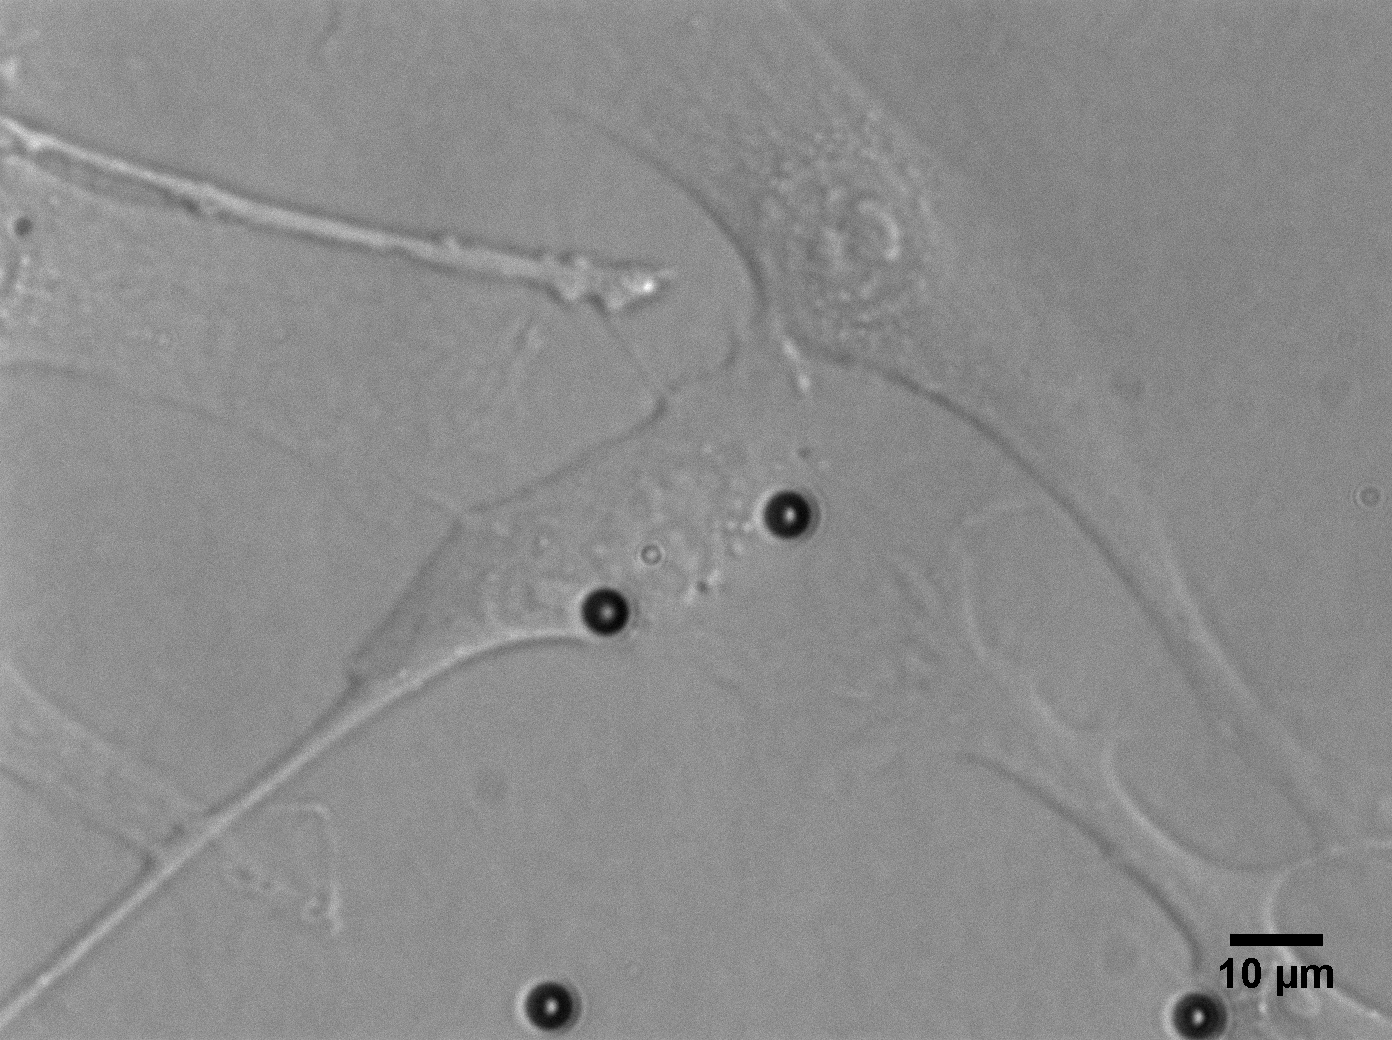
\includegraphics[scale=0.15]{c68-avt.png}
	\caption{C2C12 en culture sur du verre, avec des billes de 4,5 microns de diamètre, observées au microscope à immersion 100X.}
	\end{figure}
	
	Nous avons utilisé comme modèle une lignée immortalisée de myoblastes murins de l'ATCC, les C2C12. Elles présentent l'avantage d'être la lignée immortalisée la plus proche des cellules qui sont utilisées par nos partenaires de l'Institut Cochin dans leurs expérimentations animales sur les souris. 
	
	Ce sont des cellules adhérentes qui conservent leur capacité à se différencier en myotubes lorsqu'elles atteignent la confluence et sont placées dans un milieu pauvre en sérum. C'est pourquoi il est essentiel de les maintenir en permanence en-dessous de la confluence. 
	
	Elles adoptent des formes variées (allongées, triangulaires, en disque) et se déplacent sur leur surface de culture en étendant des lamellipodes. 
	
	Les C2C12 sont cultivées dans un milieu de culture composé de DMEM (Dulbecco's Modified Eagle Medium) à 4,5g/L de L-Glucose supplémenté de 10\% de Sérum de Veau F\oe tal (SVF) et de 1\% d'antibiotiques (Pénicilline et Streptomycine dans un incubateur à 37\degres   C et 5\% de CO$_2$. 
	
	
	Lorsqu'elles sont proches de la confluence, il faut rincer deux fois les cellules avec du PBS (Phosphate Buffered Saline) et les laisser incuber 5 minutes à 37\degres   C dans un mélange Trypsine/EDTA. La trypsine est une enzyme qui va casser les adhésions cellulaires, tandis que l'EDTA joue le rôle de chélateur des ions calcium qui sont indispensables pour créer des adhésions. Une fois les cellules décollées, elles sont diluées dans du milieu de culture qui inactive la trypsine et ensemencées à nouveau sur des boîtes de culture. Cette opération s'appelle le passage. 
	 
	\subsection{Culture sur PDMS ou sur verre  \label{Coating}}

	Pour réaliser les différentes expériences de rhéologie cellulaire, les cellules doivent être cultivées sur d'autres substrats que dans les boîtes de cultures : sur des lamelles de verre carrées (22mmm x 22mm x 100 \micro m) dans le cas des pinces magnétiques et sur des disques de PDMS (30mm de diamètre et 0.3 mm d'épaisseur) dans le cas de l'étirement. 
	
	Les disques de PDMS doivent préalablement être passées dans un four à plasma pendant 2 minutes afin de rendre leur surface hydrophile. Cette opération stérilise également les disques. Les lamelles de verre doivent être stérilisées 30 minutes à l'aide d'un rayonnement UV. 
	
	Les lamelles comme les disques sont placés dans les puits d'une plaque 6 puits, et mis à incuber 30 minutes à 37\degres   C dans 1ml de milieu complet et 5\micro g de fibronectine qui va s'adsorber sur la surface. 
	
	Après rinçage, \nombre{110 000} cellules sont ensemencées sur chaque lamelle dans du milieu complet. 
	
	\subsection{Visualiser une protéine dans la cellule : anticorps, marqueurs et protéines fluorescentes}
	
	Trois techniques ont été utilisée pendant cette thèse pour visualiser nos deux protéines d'intérêt, l'actine et MRTF, dans les cellules. 
	
	La première et la plus ancienne fait appel à des anticorps spécifiquement dirigés contre la protéine cible. Une fois que les anticorps se sont fixés sur leurs cibles, un anticorps secondaire couplé à un fluorophore vient détecter et se fixer sur le premier anticorps. 
	
	La seconde fait appel à des molécules spécifiquement dirigées contre notre protéine d'intérêt et couplées à un fluorophore. C'est le cas par exemple de la phalloïdine, drogue issue de l'Amanite Phalloïde qui a la propriété de se fixer aux filaments d'actine.	
	
	La dernière technique fait appel à la Green Fluorescent Protein (GFP), protéine découverte dans les années soixante chez une méduse, et utilisée à partir des années 90 pour marquer des protéines. En fusionnant la séquence génétique de la GFP avec la séquence de la protéine à observer, on obtient un nouveau gène codant pour une version fluorescente de la protéine d'intérêt. Après introduction du gène dans les cellules, celles-ci expriment alors la version fluorescente de la protéine. Cette utilisation de la GFP a révolutionné la biologie cellulaire et a été l'objet du prix Nobel de Chimie en 2008. Aujourd'hui, il existe de nombreuses variantes de cette technique, que ce soit au niveau des bandes d'émission et d'absorption du fluorophore (il en existe de toutes les couleurs du spectre visible) ou au niveau de la manière dont le gène de la nouvelle protéine est intégrée dans les cellules (transfection, électroporation, infection par des virus  \dots).
	
	Cette dernière technique permet d'observer la protéine fluorescente en direct pendant la vie de la cellule, alors que la première technique ne peut être utilisée que sur des cellules fixées. La seconde technique peut parfois être utilisée sur des cellules vivantes lorsque la drogue utilisée n'est pas trop toxique. 
	
	\subsubsection{Visualiser le cytosquelette d'actine dans le cadre des expériences sur MRFT-A}
	
L'observation en direct du cytosquelette d'actine est particulièrement intéressant car le système est très dynamique, ce que ne peuvent pas capturer les expériences sur cellules fixées.
Cependant, cela signifie qu'il faut trouver un moyen d'observer l'état du cytosquelette en le perturbant le moins possible. 

Durant cette thèse, j'ai testé quatre moyens d'observer l'actine ou les filaments d'actine dans les cellules vivantes. Tous se sont finalement révélés perturber dans une certaine mesure l'état du cytosquelette. 

La première méthode d'observation de l'actine dans les cellules vivantes est de leur faire exprimer, en plus de l'actine endogène, un autre gène codant pour une actine fluorescente, en l'occurence ici une actine dotée d'un fluorophore mCherry. 
Elle a l'avantage de marquer toute l'actine, et pas seulement les filaments comme les méthodes qui seront présentées après. 
Mais elle a le désavantage de faire sur-exprimer l'actine	 à la cellule, de manière variable d'une cellule transfectée à l'autre. 
Or MRTF-A est une sonde extrêmement sensible de la quantité de G-actine dans la cellule.  Sur-exprimer l'actine augmente la quantité totale d'actine G, et a un effet très visible sur MRTF-A, comme il sera présenté au chapitre 8. 

Les trois autres méthodes sont des détecteurs qui marquent uniquement les filaments d'actine, avec l'avantage de voir plus nettement la structure du cytosquelette. Il est à noter qu'actuellement il n'existe aucune sonde commercialisée pour observer l'actine monomérique \textit{in vivo}, même si une sonde a été développée récemment à partir des groupes RPEL de MRTF-A \parencite{belin_visualization_2013}. 

La LifeAct est une petite protéine de seulement 17 acides aminés qui se lie aux filaments d'actine \parencite{riedl_lifeact:_2008}. Adjointe à un fragment de protéine fluorescente, comme la GFP ou mCherry, elle permet d'observer les filaments dans les cellules vivantes.  Son ADN doit être transfecté dans la cellule pour y être exprimé avant observation. Elle a été présentée comme un moyen s'observer les filaments sans les perturber, et sans affecter leur polymérisation et leur dépolymérisation. Cependant, et comme ce sera présenté au chapitre 8, la LifeAct n'est pas complètement sans influence sur le cytosquelette d'actine. On constate une tendance à stabiliser les filaments d'actine qui est visible par l'observation de MRTF-A. 

La F-tractin \parencite{johnson_neuronal_2009} est un fragment de protéine constitué des 66 premiers acides aminés de l'inositol trisphosphate 3-kinase A, qui se lie aux filaments d'actine. Comme la LifeAct, sa séquence codante doit être exprimée par la cellule avant observation. Comme la Life, j'ai également observé une tendance de la F-tractin à stabiliser suffisamment les filaments d'actine pour affecter la localisation de MRTF-A. 

Enfin, la SiRactine est une des dernières sondes développées pour marquer les filaments d'actine \textit{in vivo} \parencite{lukinavicius_fluorogenic_2014}. Il s'agit d'un fluorophore Silicone-Rhodamine conjugué à un fragment de la japlakinolide, drogue connue pour se lier aux filaments d'actine et les stabiliser. Cette construction a pour particularité, par un mécanisme d'activation, d'être 100 fois plus fluorescentes lorsqu'elle est liée aux filaments d'actine que dans l'état non-lié, ce qui minimise le bruit de fond. La qualité de la fluorescence devait permettre d'utiliser la SiR-actine dans des quantité suffisamment faibles pour que l'influence stabilisatrice du japlakinolide sur les filaments d'actine soit invisible. Un effet sur les expériences avec MRTF-A est néanmoins visible. 

MRTF-A est une sonde extrêmement sensible de l'état du cytosquelette de la cellule, et toutes les méthodes que nous avons utilisées pour visualiser le cytosquelette \textit{in vivo} ont montré des effets sur sa localisation dans une population de cellules. 
	
	
	\subsection{Transfections}
	Afin de visualiser les protéines qui nous intéressent, on ajoute aux cellules de l'ADN non chromosomique d'origine bactérienne appelés plasmides qui codent pour une version fluorescente de nos protéines d'intérêt. Ces plasmides sont intégrées aux cellules grâce à des agents spécifiques comme la nanofectine et la lipofectamine lors de la transfection. 
	
	\begin{figure}
	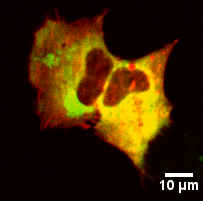
\includegraphics[scale=0.75]{C2C12_RGB-1.png}
	\caption{C2C12 transfectées avec un plasmide MRTF-A GFP (en vert) et un plasmide Actine Mcherry (en rouge)}
	\end{figure}
	
	Les cellules transfectées expriment donc deux versions de la protéine : la version endogène qui se trouve dans leur propre génome, et la version fluorescente du plasmide. La protéine que l'on observe est par conséquent toujours surexprimée par rapport à la situation normale, d'un facteur qui peut être variable d'une cellule à l'autre, selon la quantité de plasmide qui a été intégrée par la cellule : certaines cellules n'ont incorporé aucun plasmide et ne sont donc pas fluorescentes, d'autres en ont incorporé une grande quantité et sont très fluorescentes. 
	
	La transfection est d'autant plus efficace que les cellules sont proches de la confluence. Cependant, on ne peut pas laisser les C2C12 atteindre la confluence, l'efficacité de transfection est donc toujours limitée. La transfection peut se faire avant ou après l'ensemencement des cellules sur leur substrat (verre ou PDMS selon l'expérience). Lorsque la transfection a lieu avant l'ensemencement, elle est faite directement dans la boîte de culture, alors que lorsqu'elle est faite après, elle a lieu dans les puits. 
	
	 
	
	\subsubsection{Protocole de transfection}
	
	Dans les protocoles suivants, les proportions sont données pour un puits d'une plaque 6 puits. Une petite boîte de culture (T-25) représente une surface de 2,5 fois celle d'un puits, les quantités utilisées lors de la transfection d'une boîte sont donc multipliées d'autant.
	
	Trois protocoles sont décrits simultanément ici : le protocole pour une transfection simple de MRTF-A GFP , puis pour une transfection double MRTF-A GFP/Actine Mcherry (option 1) ou MRTF-A GFP/LifeAct RFP (option 2). Sauf indication contraire, toutes les étapes et ingrédients optionnels sont en plus des ingrédients pour la transfection simple.
	
\paragraph{Ingrédients :}
\begin{quote}

	\begin{itemize}
	\item Des C2C12 ensemencées dans un puits d'une plaque 6 puits
	\item 1 \micro g de nanofectine (PAA Nanofectin Kit)
	\item 1 \micro g d'ADN de MRTF-A GFP
	\item (option 1 : Actine Mcherry) 1 \micro g d'ADN d'Actine Mcherry
	\item (option 1 : Actine Mcherry) 1 \micro g de nanofectine
	\item (option 2 : LifeAct RFP) 0,75 \micro g d'ADN de LifeAct RFP
	\item (option 2 : LifeAct RFP) 0,75 \micro g de nanofectine
	\item 2*50 \micro l de NaCl 150mM
	\item (option 1 ou 2) 2*50 \micro l de NaCl 150mM
	\item 0,9ml de milieu complet (transfection simple uniquement)
	\item (option 1 ou 2) 0,8 ml de milieu complet
	\end{itemize}
\end{quote}

\paragraph{Protocole : }
\begin{quote}
\begin{enumerate}
	\item Diluer dans un eppendorf 1 \micro g de MRTF-A GFP dans 50 \micro l de solution de NaCl 150mM. 
	\item Diluer de même 1 \micro g de nanofectine
	\item (option 1 ou 2 ) Répéter ces deux étapes avec l'Actine Mcherry ou la LifeAct RFP
	\item Transvaser le contenu de l'eppendorf de nanofectine dans l'eppendorf d'ADN (le sens est important)
	\item (option 1 ou 2 ) Répéter l'opération pour les deux autres tubes
	\item Laisser incuber 30 minutes à 37~\degres C 
	\item Transvaser le ou les mélange(s) nanofectine + ADN dans du milieu complet de façon à obtenir 1  ml de solution
	\item Rincer les cellules
	\item Ajouter le mélange nanofectine + ADN + milieu complet sur les cellules
	\item Laisser incuber à 37 \degres C pendant au moins 6 heures
	\item Enlever le mélange, rincez et remplacez avec du milieu complet
	\item Laisser les cellules exprimer le plasmide entre 12 et 24h après rinçage
\end{enumerate}
\end{quote}

	\subsection{Marquage DAPI sur cellules vivantes}
	
	Le  4',6'-diamidino-2-phénylindole (DAPI) est une molécule fluorescente qui peut se fixer entre les bases A et T de l'ADN. Elle peut entrer dans les cellules vivantes et permet ainsi de marquer l'ADN du noyau. Sa localisation dans l'ADN perturbe la réplication de l'ADN nécessaire à la division cellulaire, c'est pourquoi le DAPI est ajouté à la dernière minute avant les expériences sur cellules vivantes. 
	
	Trente minutes avant l'observation, du DAPI est ajouté au milieu de culture en proportion 1/1000 ou 1/500 (selon l'efficacité du lot de DAPI pour entrer dans les cellules). Il est si possible rincé avant l'observation pour améliorer le contraste. 
	\subsection{Fixation}
	La fixation permet de figer les protéines des cellules à un instant donné. Elle est réalisée en ajoutant sur une lamelle recouverte de cellules préalablement rincée au PBS une solution à 4\% de paraformaldéhyde (PFA) pendant 20 minutes à température ambiante. Cette solution est ensuite rincée au PBS. 
	
	Les lamelles fixées ainsi obtenues peuvent être conservées plusieurs mois à 4\degres   C et observées longuement au microscope. 
	\subsection{Marquages sur cellules fixées}
	Les cellules fixées peuvent être marquées par des molécules fluorescentes qui peuvent être perturbatrices ou toxiques pour des cellules vivantes. Ici nous avons réalisé sur cellules fixées des marquages à 4 couleurs : rouge profond pour les filaments d'actine, rouge pour l'actine monomérique, vert pour la MRTF-A et bleu pour l'ADN. 
		\subsubsection{Perméabilisation}
		Afin de faire rentrer les molécules et protéines qui vont nous permettre de marquer les protéines des cellules, il est nécessaire de perméabiliser les cellules. Pour cela, on va ajouter aux cellules fixées une solution contenant 0.5\% de Triton, un tensio-actif qui va permettre de créer des trous dans les membranes plasmiques des cellules fixées. 
		Pour améliorer la spécificité des différents marqueurs on va également saturer les sites de liaison des protéines à l'aide de protéines non spécifiques : Bovine Serum Albumine (BSA) 4\% et Horse Serum (HS) 5\%. 
		
		Les lamelles de cellules fixées sont donc initialement laissées 3h à température ambiante dans la solution de saturation composée de 0.5\% triton, 5\% HS et 4\% BSA. 
		
		\subsubsection{Phalloïdine}
		La phalloïdine est une drogue issue de l'amanite phalloïde qui se lie aux filaments d'actine et les stabilise. Utilisée \emph{in vivo} elle perturbe significativement le cytosquelette jusqu'à se révéler toxique pour les cellules. 
		
		Sur des cellules fixées, la phalloïdine permet de marquer spécifiquement les filaments d'actine. La phalloïdine   utilisée pendant nos marquages a été ajoutée aux cellules fixées la veille de l'observation et laissée toute la nuit à 4\degres C, et rincée avant observation. 
		\subsubsection{DNaseI}
		La DNaseI est une protéine naturellement présente dans le noyau des cellules et qui découpe l'ADN en morceaux de 4 paires de bases. Son action est bloquée lorsqu'elle est liée à un monomère d'actine. En raison de son action sur l'ADN, elle ne peut pas être utilisée sur des cellules vivantes. Sur des cellules fixées, elle est un marqueur spécifique du monomère d'actine. 
		
		Comme la phalloïdine, elle est ajoutée aux cellules fixées la veille de l'observation et laissée toute la nuit à 4\degres   C. 
		\subsubsection{MRTF-A endogène}
		
		Lorsque les cellules sont fixées, on peut observer la MRTF-A endogène grâce à l'immunofluorescence plutôt que de transfecter de la MRTF-A GFP dans les cellules. Cela nous permet de détecter les protéines sauvages exprimées directement par cellule sans surexpression induite par la transfection. 
		
		Le marquage se fait en deux étapes : le marquage par un anticorps spécifique anti-MRTF-A, puis le marquage de l'anti-corps anti-MRTF-A par un autre anti-corps qui est fluorescent. L'anti-corps primaire est placé pendant 30 minutes à température ambiante. La lamelle est ensuite rincée et on y ajoute l'anticorps secondaire à nouveau pendant 30 minutes à température ambiante, puis on rince à nouveau. 
		 
				
		\begin{figure}
		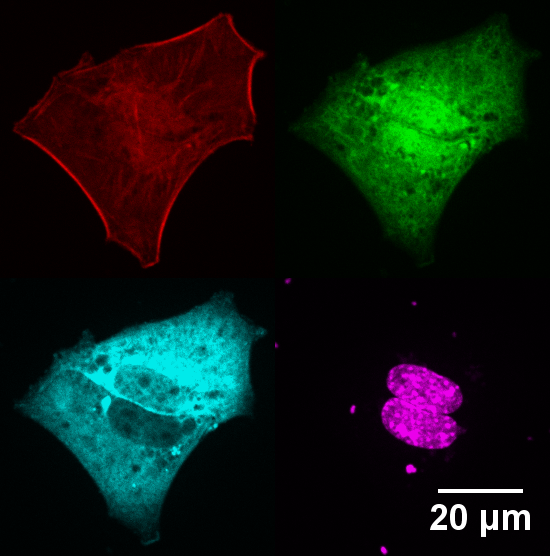
\includegraphics[scale=0.4]{Montage_sc.png}
		\caption{C2C12 transfectées MRTF-A GFP (ici en cyan), fixées et marquées phalloïdine Alexa647 (ici en rouge), DNAseI Alexa547 (ici en vert) et DAPI (ici en magenta)}
		\end{figure}

\subsubsection{Protocole de marquage quadrichrome}
\paragraph{Durée estimée : 3h + 3*30 minutes + une nuit }
 \paragraph{Ingrédients pour une lamelle : }
 \begin{quote}
 
 
 \begin{itemize}
 \item une lamelle de cellules fixées
 \item PBS
 \item 40 \micro g de BSA
 \item 50 \micro l de Horse Serum
 \item 5 \micro l de Triton
 \item 4 \micro l de Phalloïdine Alexa 647 (Life Technologies) 6.6 \micro M dans le méthanol
 \item 1 \micro l de DNase I Alexa 594 (Life Technologies) 161 \micro M dans un mélange 50\% v/v PBS 50\% glycérol
 \item 4 \micro l d'anticorps MRTF-A H140 (Santa Cruz Biotechnology) 200\micro g/ml dans PBS 0.1\% gélatine
 \item 2 \micro l d'anticorps goat anti-rabbit Alexa 488 (Jackson ImmunoResearch) 1.5mg/ml dans de l'eau diluée
 \item 1 \micro l de DAPI
 \end{itemize}
\end{quote}

\paragraph{Protocole pour une lamelle : }
\begin{enumerate}
\item Mélanger 40 \micro g de BSA, 50 \micro l de HS et 5 \micro l de Triton dans 905\micro l de PBS. Le mélange constitue la solution de perméabilisation et de saturation.
\item Enlever le PBS de la lamelle fixée
\item Ajouter la solution de saturation sur la lamelle, et laisser incuber 3h à température ambiante
\item Ajouter 4 \micro l d'anti-MRTF-A H140 à 996 \micro l de PBS
\item Enlever la solution de saturation de la lamelle
\item Ajouter l'anti-MRTF-A diluée et laisser incuber 30 minutes à température ambiante
\item Enlever l'anticorps et rincer deux fois au PBS
\item Ajouter 2 \micro l d'anti-rabbit Alexa 488 dans 998 \micro l de PBS
\item[Attention] à partir de cette étape, pour limiter le photo-blanchiment, il faut éclairer la lamelle le moins possible. Pendant les temps d'incubation, elle doit être protégée par un film opaque. 
\item Ajouter l'anti-rabbit diluée sur la lamelle et laisser incuber 30 minutes à température ambiante
\item Enlever l'anticorps et rincer 2 fois au PBS
\item Ajouter 1 \micro l de DAPI à 999 \micro l de PBS
\item Ajouter le DAPI dilué sur la lamelle et laisser incuber 30 minutes à température ambiante
\item Enlever le DAPI et rincer 2 fois à température ambiante
\item Ajouter 4 \micro l de phalloïdine et 1 \micro l de DNase I à 995 \micro l de PBS
\item Ajouter le mélange phalloïdine et Dnase diluées à la lamelle et laisser incuber toute la nuit.
\item Rincer deux fois avec 1ml de PBS. Les lamelles marquées peuvent être conservées plusieurs semaines à 4\degres C dans l'obscurité, mais la qualité du signal décroît avec le temps, il est donc préférable de les observer le lendemain du marquage.

\end{enumerate}

\section{Pinces magnétiques}

Les pinces magnétiques sont destinées faire de la rhéologie à l'échelle locale sur une cellule unique. Comme les pinces optiques, elles utilisent des billes micrométriques recouvertes de protéines d'adhésion pour s'ancrer à la cellule. 
Une force exercée sur la bille sera alors transmise par les adhésions à la cellule.
 Les contraintes sont donc non seulement ressenties mécaniquement par la cellule, mais aussi biochimiquement au niveau des protéines des complexes d'adhésions. 
La bille, observée au microscope, se déplace en réponse à la force, mais est retenue par la cellule.

Pour étudier la rhéologie cellulaire, on va alors exercer une force connue sur la bille, et mesurer au microscope son déplacement, et donc la déformation de la cellule.
Nous nous sommes placés ici en régime de fluage, plus adapté à la pince magnétique. La bille exerce une contrainte constante sur la cellule $\sigma_0$, qui est reliée à la déformation de la cellule par la relation : 
$$\epsilon (t) = \sigma_0 J(t)$$.

Un modèle nous permet de relier la contrainte subie par la cellule $\sigma_0$ à la force exercée par l'électro-aimant sur la bille $F_0$ et la déformation de la cellule $\epsilon (t)$ au déplacement de la bille $x(t)$. 






Les pinces magnétiques ont été construites pour contourner un certain nombre de limitations que rencontraient les pinces optiques qui existaient déjà au laboratoire, en particulier pour exercer des forces plus grandes pendant des durées plus longues et des découpler l'observation et l'application de force, qui se faisaient par l'intermédiaire de l'objectif dans le cas des pince optiques. Cela s'est fait au prix de la perte de contrôle de la direction de la force : la pince magnétique ne peut que tirer la bille vers la pointe, dans la direction de l'axe de l'électro-aimant. 


	\subsection{Description}
		\subsubsection{Principe}
		Lorsqu'on applique un champ magnétique $$\vec{H} = \frac{\vec{B}}{\mu}$$ sur une bille paramagnétique de volume $V$ et de susceptibilité magnétique $\chi$, cela induit dans la bille un moment magnétique $$\vec{m} = \chi V \vec{H}$$ Si le champ magnétique est de plus inhomogène, la bille subit alors une force :$$\vec{F} = \left( \vec{m}. \vec{\nabla} \right) \vec{B}$$
	
Le principe des pinces magnétiques est donc d'utiliser un électro-aimant, qui va créer un champ et un gradient de champ magnétiques lorsqu'il est alimenté par un courant, pour exercer des forces à distance sur un bille magnétique fixée à la cellule par des protéines d'adhésion. 	 
	 
	 
	 Afin d'exercer cette force, il est nécessaire de construire un électro-aimant répondant à plusieurs contraintes : il doit être capable de créer un fort champ magnétique ainsi qu'un fort gradient de champ magnétique, cependant il ne doit pas chauffer l'échantillon afin de ne pas endommager les cellules vivantes sur lesquelles on manipule, et cela sans système de refroidissement qui risquerait d'introduire un bruit mécanique trop important. L'électro-aimant doit pouvoir être amené le plus près possible de l'échantillon afin d'exercer une force maximale, le plus précisément possible afin de conserver une bonne précision sur la direction et la valeur de la force exercée. On souhaite manipuler avec une chambre expérimentale fermée pour éviter toute contamination des cellules, et pouvoir faire des observations en fluorescence. On souhaite également faire des expériences de longue durée, en imposant des paliers de force pendant plusieurs minutes et répétés pendant plusieurs dizaines de minutes.	
	
		\subsubsection{Billes superparamagnétiques}
		
		\begin{figure}
		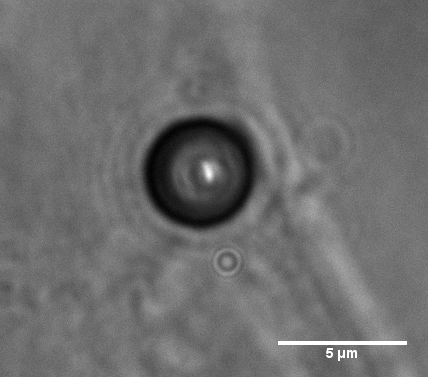
\includegraphics[scale=0.4]{Bille.PNG}
		\caption{Bille Dynabeads M-450 observée en grossissement 150X. }
		\end{figure}
		Les billes utilisées sont des Dynabeads M-450 Epoxy d'Invitrogen Dynal AS, Oslo, Norvège. 
		Ce sont des billes de polystyrène sphériques, de 4,5$\mu$m de diamètre, recouvertes en surface de groupes epoxy afin de permettre l'ajout de ligands en surface, et contenant des nanoparticules d'oxydes de fer qui leur confèrent leurs propriétés superparamagnétiques. 
		Elles sont initialement fournies dans une suspension concentrée ($4.10^8$ billes/ml) dans de l'eau distillée. On les recouvre de fibronectine pour une fixation spécifique aux intégrines.
		Pendant les expériences de pinces magnétiques, la bille magnétique par l'intermédiaire de laquelle on applique une force sur la cellule est observée au microscope à l'aide d'un objectif 100X et filmée pendant toute la durée de l'expérience.  Ces images sont ensuite traitées avec un logiciel d'analyse d'image (ImageJ, National Institue of Health) qui ajuste une ellipse sur l'image des billes. Le logiciel nous donne pour chaque image de chaque expérience le grand axe et le petit axe de l'ellipse ajustée. Une bille est donc mesurée environ \nombre{4 000} fois pendant une expérience.  
		Nous obtenons donc \nombre{385 885} mesures de taille pour 191 billes observées pendant 191 expériences de pinces, avec une taille moyenne de 4.4067 $\pm$ 0.0002 \micro m et un rapport petit axe sur grand axe $e=0.98585 \pm 0.0008$. Les billes apparaissent donc légèrement plus petites qu'annoncé par le fabriquant mais semblent bien sphériques.
		\begin{figure}
		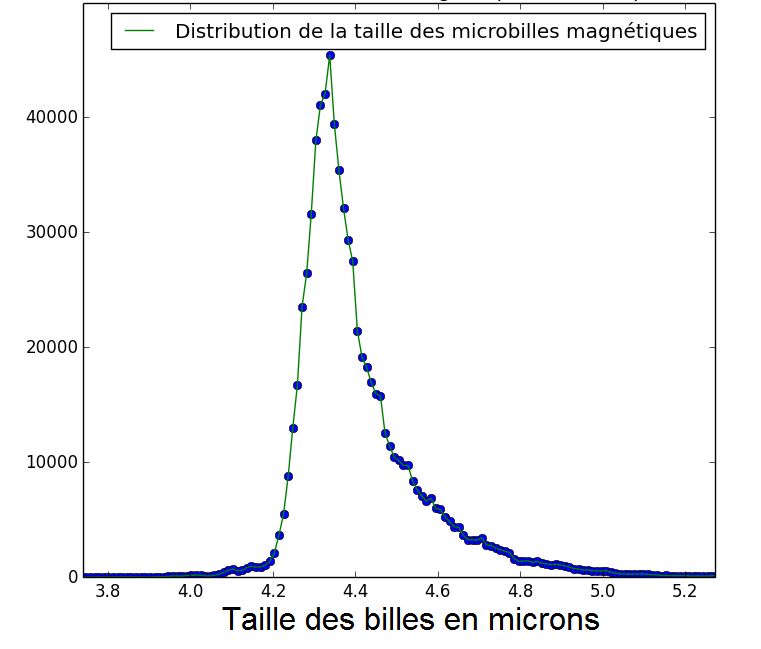
\includegraphics[scale=0.3]{Taille_des_billes.png}
		\caption{Fonction de distribution de taille des billes magnétiques utilisées dans \nombre{191} expériences de pinces. Pour chaque expérience, lorsque la bille est suivie par le logiciel d'analyse d'image, son grand axe et son petit axe sont mesurés pour chaque temps. La fonction est asymétrique car lorsque la bille n'est pas tout à fait au point, son diamètre apparaît plus grand.}
\end{figure}		 
		
		\subsubsection{\'Electroaimant}
		L'électro-aimant est composé d'un c\oe ur entouré d'une bobine de fil de cuivre. Le passage d'un courant électrique dans la bobine crée un champ magnétique dont les lignes de champ sont conduites par le c\oe ur. 
		
		\paragraph{Le c\oe ur} Deux types de c\oe ur ont été testés : un c\oe ur en fer doux (diamètre : \nombre{5.30}mm, longueur : \nombre{52.17}mm) et un c\oe ur en mu-métal, un alliage de grande perméabilité magnétique (diamètre : \nombre{5,10mm} , longueur : \nombre{143,64}mm).
		
		Une extrémité du barreau est taillée en pointe. La forme de pointe permet d'augmenter le gradient de champ magnétique en resserrant les lignes de champ à cet endroit. Il est très important de conserver sa symétrie cylindrique, et d'avoir le rayon de courbure le plus faible possible au bout de la pointe. Les résultats obtenus sont visible en figure $\ref{pointe}$. \'Etant en fer doux, le barreau est très malléable, il faut donc le manipuler avec précautions : le moindre choc aplatit la pointe. 
	 Le barreau a été usiné au tour à l'atelier de mécanique, puis pour la taille d'entretien de la pointe, on monte le barreau sur une perceuse sur pied, ce qui permet de garder la symétrie cylindrique, et on l'approche d'un morceau de papier de verre de grain de plus en plus fin, collée sur une pièce métallique inclinée avec un angle de 30 $\degres$ .
	 
	 \begin{figure}[ht!]%
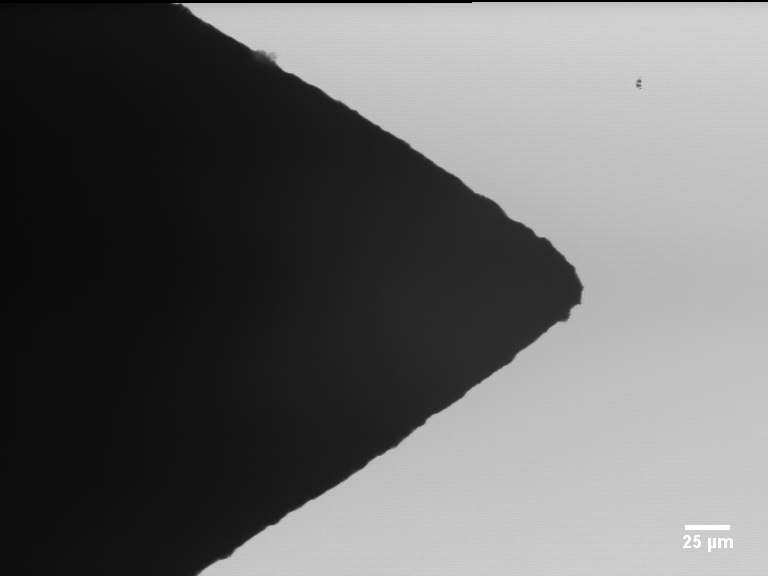
\includegraphics[width=6cm]{pointe1-2011-03-29-20X.png}%
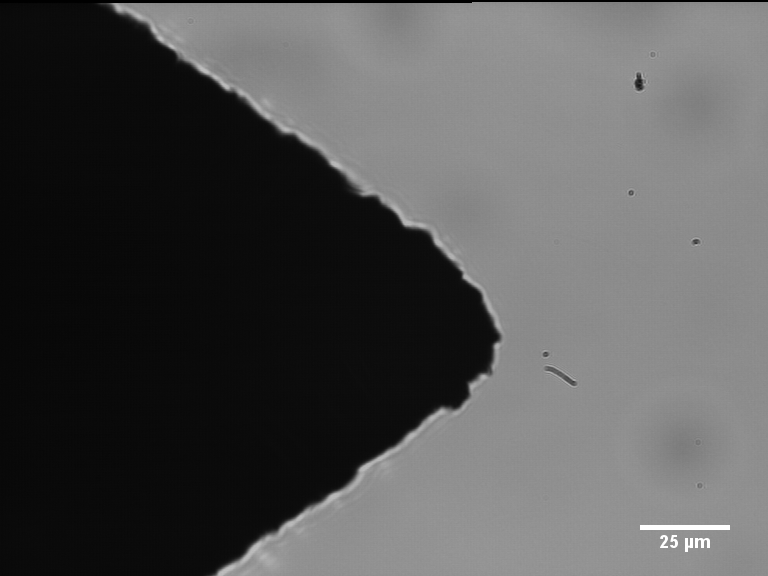
\includegraphics[width=6cm]{pointe1-2011-03-29-40X.png}
\caption{À gauche une image de la pointe en fer doux au grossissement X20. À droite, la même pointe au X40. Le rayon de courbure mesuré est de l'ordre de 2
0$\mu$m.}%
\label{pointe}
\end{figure}
	 
	 L'angle optimal pour maximiser le gradient peut être calculé \parencite{durand_electrostatique_1953}, il vaut environ 55\degres. Ici, on doit aussi prendre en compte le fait que la pointe doit être approchée de biais au-dessus de la lamelle d'échantillon. Il nous faut donc un angle plus faible que l'angle optimal, trop obtus. On a fixé cet angle à 30 $\degres$ , car il est prévu d'approcher la pointe de la lamelle sur laquelle seront les cellules avec un angle de 45 $\degres$, comme représenté sur la figure \ref{montage global} .

\paragraph{La bobine}

	L'optimisation des caractéristiques de l'électro-aimant a été l'objet de mon stage de Master 2. 
	Deux contraintes s'opposent lors de la fabrication : l'augmentation du champ magnétique et l'effet Joule. 
	
	\begin{figure}
	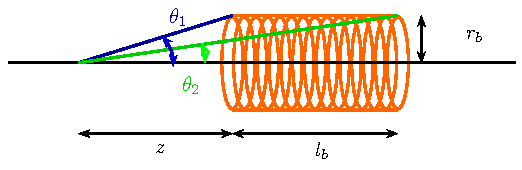
\includegraphics[scale=1]{champB.pdf}
	\end{figure}
	Le champ $\vec{B}$ généré par un solénoïde de longueur finie dans le vide sur son axe à une distance $z$ vaut:
		
		$$ \vec{B} = \frac{\mu_0 n I}{2} \left(\cos \left(\theta_2 -\cos \theta_1 \right)\right) \vec{u_z}$$
		
		Sa valeur dépend du nombre $n$ de spires par mètre, de la longueur de la bobine $l_b$, de son rayon $r_b$ et du courant $I$ qui la traverse. On veut donc maximiser $n$ et $I$ pour augmenter la valeur de $B$. La distance $z$ sera de l'ordre de 700\micro m. 
		
		La puissance dissipée par effet Joule $$P = R I^2$$ dépend de la résistance de la bobine et de $I$, il s'agit de minimiser ces quantités.
		
		La résistance $R$ de la bobine dépend de la section du fil $s$, de sa longueur totale $L$ et de $\gamma$ la conductivité du cuivre :
:
		 $$R = \frac{L}{\gamma s}$$
		
				
		Le nombre de spires par mètre est directement reliée à la section du fil   : $$ n = \frac{1}{2r_f} = \frac{1}{2 \sqrt{\frac{s}{\pi}}} = \sqrt{\frac{\pi}{4s}}$$  Il est facile de voir que lorsque $s$ augmente, $R$ diminue en $s^{-1}$ alors que $n$ ne diminue qu'en $s^{-1/2}$, et donc qu'il faut choisir la section de fil la plus grande disponible.
		En pratique, on ne fait pas qu'une couche de bobinage, mais $n_c$, le nombre de spires par mètres est aussi relié à la longueur totale de fil $L$.
		
		$$R \propto L \approx n_c \frac{\pi r_b l_b}{r_f}$$ où  $l_b$ sa longueur, $r_f$ le rayon du fil. 
		
		$$n = n_c \frac{1}{2r_f}$$
		
		Pour augmenter $n_c$ en augmentant le moins possible $R$, il faut alors minimiser le rapport $\frac{\pi r_b l_b}{r_f}$. On a choisi $r_f$ le plus grand disponible, on prend également $r_b$ le diamètre de la bobine le plus petit possible.
		
		En ce qui concerne la longueur de la bobine, $l_b$, on aimerait la minimiser pour diminuer $R$, cependant, le champ $B$ est maximal pour une bobine de longueur infinie. La longueur optimale correspond en fait à celle du c\oe ur : ajouter de la longueur de bobine au-delà n'augmente que peu le champ, à cause de la faible perméabilité magnétique de l'air.
		
		La bobine finalement utilisée dans nos expériences est composée de 8 couches de fil de cuivre de diamètre 0,5mm bobinées sur un tube d'aluminium de diamètre extérieur égal à 5,38mm sur une longueur de 66,5mm et de diamètre intérieur égal à celui du c\oe ur. Sa résistance est mesurée à 3,3$\Omega$ et son inductance à 1,2mH. 
		
		L'aluminium est un bon support pour la bobine car il est à la fois léger, car il ne faut pas surcharger le micromanipulateur qui portera l'électro-aimant dans le montage final, et qu'il conduit bien la chaleur dégagée par l'effet Joule pour qu'elle soit évacuée vers le c\oe ur. L'aluminium a pu également être taraudé à une extrémité afin d'y attacher une vis de support en laiton qui est tenue par le micromanipulateur, et qui sert également à évacuer une partie de la chaleur de la pointe.                       
		\subsubsection{Montage sous microscope}
		\paragraph{Circuit électrique}
		
		Un générateur de tension basse fréquence, contrôlé par ordinateur par l'intermédiaire d'une carte PCI (Measurement Computing 1208 HS4AO), alimente un amplificateur de courant fabriqué par les ateliers du laboratoire, qui permet de délivrer des courants jusqu'à 2A à la bobine. 
		La bobine ayant à dessein une résistance la plus faible possible pour limiter l'effet Joule, une résistance de 10$\Omega$ est ajoutée au circuit. Un ampèremètre mesure à tout instant l'intensité délivrée à la bobine. 
		
		Le temps de réponse caractéristique du circuit RL est donc de 16ms, ce qui sera négligeable dans toutes les configurations où les pinces seront utilisées. 
		
		 \paragraph{Montage sous le microscope}
		 
		 \begin{figure}
		 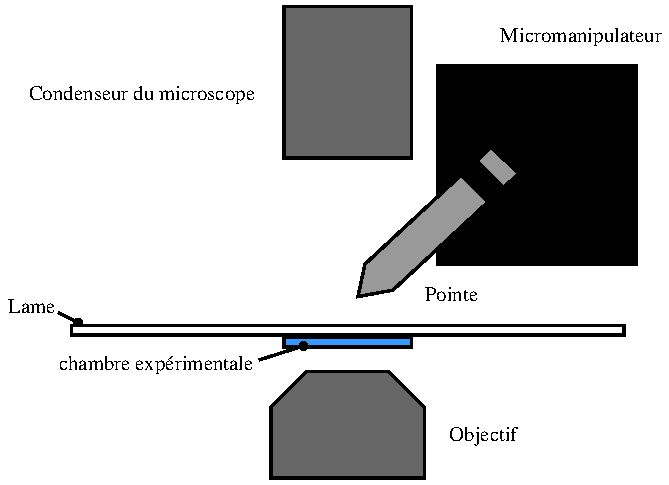
\includegraphics[scale=1]{montageglobal.pdf}
		 \label{montage global}
		 \end{figure}
		 
		 L'électro-aimant que l'on a fabriqué précédemment est monté sur un micromanipulateur (InjectMan NI2, Eppendorf, avec une précision de position de 0.1$\mu$m), incliné à 45 $\degres$ . La force que nous allons exercer sur les billes est parallèle à l'axe de la bobine, nous allons donc appliquer simultanément une force horizontale et une force verticale vers le haut. 
		 
		 Un thermomètre est fixé sur la pointe pour mesurer sa température à tout instant et vérifier qu'il n'y a pas de risque d'endommager les cellules pendant l'expérience. 
		 
		 Les cellules ont préalablement été ensemencées sur une lamelle de verre et incubées avec les microbilles recouvertes de fibronectine. Sur une lame de verre 22mm*64mm*0.15mm, on monte un séparateur (GeneFrame Spacer AB-0577, Thermo Scientific) et la lamelle de verre, le tout formant une chambre expérimentale fermée de 65\micro l emplie de milieu de culture. 		 
		 
		 Le micromanipulateur et la lamelle contenant les cellules sont montés sur un microscope inversé (Leica DMIRB). \`A l'aide du micromanipulateur, on peut approcher la pointe de l'électro-aimant à une distance de 100$\mu$m de la lamelle. On enregistre les images de la bille à l'aide d'une caméra (CoolSnap HQ2) reliée à un ordinateur qui la contrôle par l'intermédiaire de MicroManager. 
		 
		 \begin{figure}
		 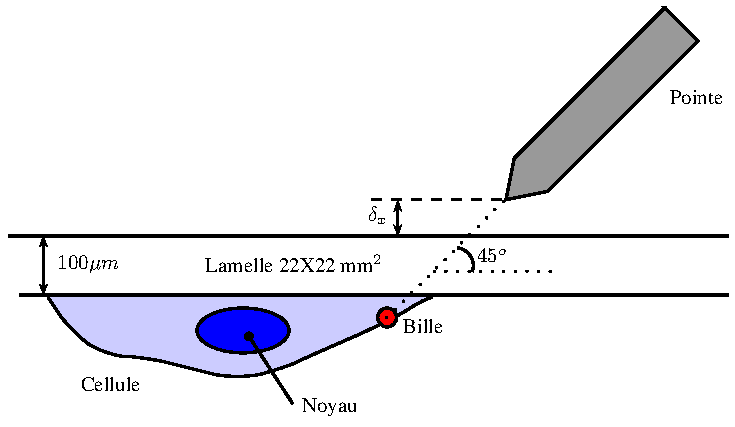
\includegraphics[scale=0.5]{modeop1.pdf}
		 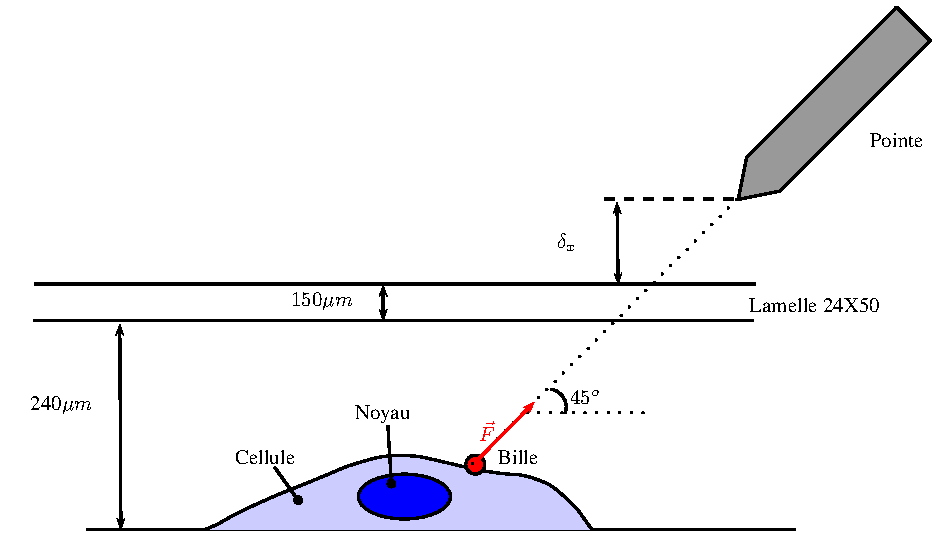
\includegraphics[scale=0.5]{modeop2.pdf}
		 \caption{Schéma des deux montages possibles de la lamelle par rapport à l'objectif et à la pince magnétique.}
		 \end{figure}
		 
		 Il existe deux possibilités de montage pour la lamelle : la lamelle sur laquelle sont les cellules peut être placée en haut, du côté de la pointe de l'électro-aimant, ou au contraire en bas, proche de l'objectif du microscope. 
		 
		 Dans le premier cas, la distance entre la pointe de l'électro-aimant et la bobine peut être réduite à 280 \micro m, ce qui permet d'exercer de grandes forces, de l'ordre du nanoNewton. Cependant, la distance entre l'objectif et les cellules est alors d'au moins 400 \micro m, et ne permet pas d'utiliser d'un objectif à immersion, nous restreignant à des grossissements inférieurs à 40X. 

		 Dans le second cas, on peut au contraire utiliser des objectifs à immersion à huile 100X, ce qui nous permet d'avoir une très bonne précision sur la position et sur les déplacements de la bille. Cependant, la distance entre la bille et la pointe est alors de 700 \micro m et il est alors possible d'appliquer au maximum des forces de l'ordre de 160 pN. 
		 
Le choix entre les deux méthodes dépend donc de la précision d'observation dont on a besoin et de la force que l'on souhaite exercer. 

		 
		 
		 		 
		  
		
		
	\subsection{Calibration}
  
 Les caractéristiques magnétiques des billes ne sont pas fournies par le fabriquant, et de plus à des distances inférieures au millimètre, la précision sur les mesures de $\vec{B}$ et $\vec{\nabla}B$ est mauvaise. 
 Il est donc impossible de calculer de manière fiable la force exercée par la pointe sur les billes à un courant et à une distance donnée.
 Pour connaître la force exercée par l'électro-aimant sur les billes en fonction de la distance et du courant, nous avons donc procédé à une calibration.
 
 \subsubsection{Principe}
 
 Les billes de diamètre $d=4.5$\micro m sont placées dans du PDMS liquide de masse volumique $\rho$ proche de celle de l'eau mais de grande viscosité $\eta=0.75$Pa.s. 
 Dans ces conditions, le nombre de Reynolds associé aux billes lorsqu'elles se déplacent à une vitesse $U$ dans le liquide vaut : $$Re = \frac{\rho U d }{\eta}=6*U*10^{-3}$$
 et donc $Re \ll 1$ tant que  $U \ll 167 m.s^{-1}$. 
 On peut donc en conclure que l'inertie est complètement négligeable devant les effets visqueux dans ces conditions. 
 
 Les billes subissent donc deux forces : la force magnétique exercée par la pointe, et les forces de friction visqueuses exercées par le fluide. 
 
 La force de friction visqueuse sur une sphère peut être modélisée par la relation de Stokes : 
 $$ \vec{F}_{vis}=- 3 \pi \eta d \vec{U} =-\vec{F}_{mag}$$
 
 Dans notre dispositif, les billes sont placées dans une chambre expérimentale de 240\micro m de hauteur formée par un séparateur, et l'influence de la lamelle supérieure ou de la lamelle inférieure ne peuvent pas être exclue. On note $h$ la distance à la lamelle la plus proche. 
 De plus, la viscosité $\eta$ du fluide est très sensible aux variations de température, or l'électro-aimant chauffe pendant l'application de la force à cause de l'effet Joule dans la bobine. 
 Comme la mesure est effectuée à une distance de 0,5 à 1mm de la pointe, celle-ci chauffe le fluide localement. 
 On a mesuré la dépendance de la viscosité du fluide en fonction de la température $a=0.0178 Pa.s/\deg C$ autour de 24\degres C. 
 
 Le modèle de Stokes est donc corrigé ainsi : 
 
 \begin{equation}
 {F}_{mag}= 3 \pi \left(\eta_{24^{o}C}-a\left(\frac{T_{fin}-T_{init}}{2} - 24\right) \right) *\left( \frac{d_{max}+d_{min}}{2} \right) * \left( 1+\frac{d}{h} \right)*\vec{U}
 \label{Stokes_corr}
 \end{equation}
 
 \subsubsection{Montage et protocole}
 
 \begin{figure}
 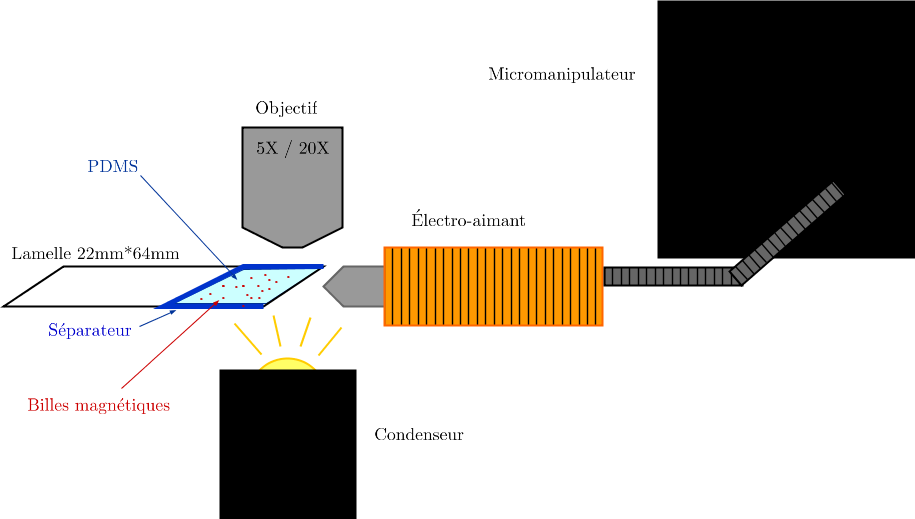
\includegraphics[scale=0.4]{Calibration_pinces.png}
 \label{calibration_pinces}
 \end{figure}
 

 
 L'électro-aimant est monté sur le micromanipulateur à l'horizontale.  
 On suspend 1 \micro l de suspension mère de billes dans 499 \micro l de PDMS, et on passe cette suspension 45 minutes dans une cuve à ultra-sons en cisaillant toutes les 5 minutes.
 La suspension est placée dans une chambre expérimentale formée par une lamelle 22mm*64mm*0.15mm, une lamelle 22mm*22mm*0.1mm et un séparateur de 240 \micro m d'épaisseur. La chambre est ouverte du côté où l'on va approcher la pointe. 
 
 La chambre expérimentale est placée sous un microscope droit Reichert doté d'un objectif 5X et d'un 20X et d'une caméra reliée à un ordinateur. Le protocole d'étalonnage est alors le suivant : 
 
 \begin{quote}
 \begin{enumerate}
 \item Placer le plan focal au centre de la chambre expérimentale selon l'axe vertical.
 \item \`A l'aide du micromanipulateur, amener la pointe à droite du champ de la caméra avec l'objectif 5X, le plus près possible de la chambre expérimentale sans entrer en contact avec le PDMS. 
 \item Prendre une image au 5X de la position de la pointe.
 \item Au 20X, repérer une bille à gauche du champ (éloignée de la pointe), l'amener dans l'axe de la pointe. 
 \item Faire le point sur la bille et repérer la hauteur du plan focal. 
 \item Relever la température de la pointe $T_{init}$.
 \item Simultanément, alimenter la bobine avec un courant continu $i$ et commencer l'acquisition à 5 images/seconde. 
 \item Lorsque la bille sort du champ de la caméra à droite, arrêter l'acquisition et couper le courant dans la bobine.
 \item Relever la température finale de la pointe $T_{fin}$.
 \end{enumerate}
 \end{quote}
 
 On recommence cette opération une dizaine de fois pour chaque intensité de courant. 
 
 \subsubsection{Traitement des données}
 On obtient alors $T_{init}$, $T_{fin}$, $i$, $h$ directement, et des vidéos desquelles on extrait $d_{min}$, $d_{max}$ les petit et grand axes de la bille, la position $(x(t),y(t))$ de la bille au cours du temps, et une image de la pointe d'où on obtient $(x_p,y_p)$ la position de la pointe. 
 
 Les vidéos des billes attirées par la pointe sont traitées avec l'algorithme d'ImageJ \emph{Analyse Particules} qui repère les billes et relève leur position sur toutes les images successives et leur taille. 
 Cependant, si ImageJ repère toutes les billes sur chaque image, il ne relie pas une position à l'instant $t$ à la position de la même bille à l'instant $t+ \Delta t$. 
 
 Pour cela, j'ai créé sous Igor un algorithme de tri qui sépare les trajectoires des différentes billes et crée pour chaque bille une trajectoire $(x(t),y(t))$. 
 
 La position de la pointe $(x_p,y_p)$ est repérée sur l'image prise en début d'expérience au 5X, grâce à ImageJ également. Comme la position du champ du 20X dans le champ du 5X est connue, la position $(xp,yp)_{5X}$ de la pointe dans le champ du 5X peut être convertie en position dans le champ du 20X $(xp,yp)_{20X}$. 
 
 Nous nous situons toujours dans le régime stationnaire $\vec{F}_{mag}=-\vec{F}_{vis}$. 
 Les billes ne se déplacent cependant pas à une vitesse constante, car lorsqu'elles se rapprochent de la pointe, la force $F_{mag}$ à laquelle elle sont soumises augmente. 
 
 Enfin, pour chaque bille, un algorithme sous Igor permet de : 
 \begin{itemize}
 \item Calculer la distance de la bille à la pointe à chaque instant.
 \item \`A l'aide d'un ajustement linéaire local de la trajectoire sur quarante points (donc 8 secondes), en déduire la vitesse $U(t)$ de la bille.
 \item \`A l'aide de la formule de Stokes corrigée \ref{Stokes_corr}, estimer la force exercée par la pointe sur la bille.
 \end{itemize}
 
 On obtient donc une série de courbes de calibration, où à chaque intensité de courant on connaît le module de la force magnétique $F$ en fonction de la distance de la bille à la pointe. 
 
 \begin{figure}
 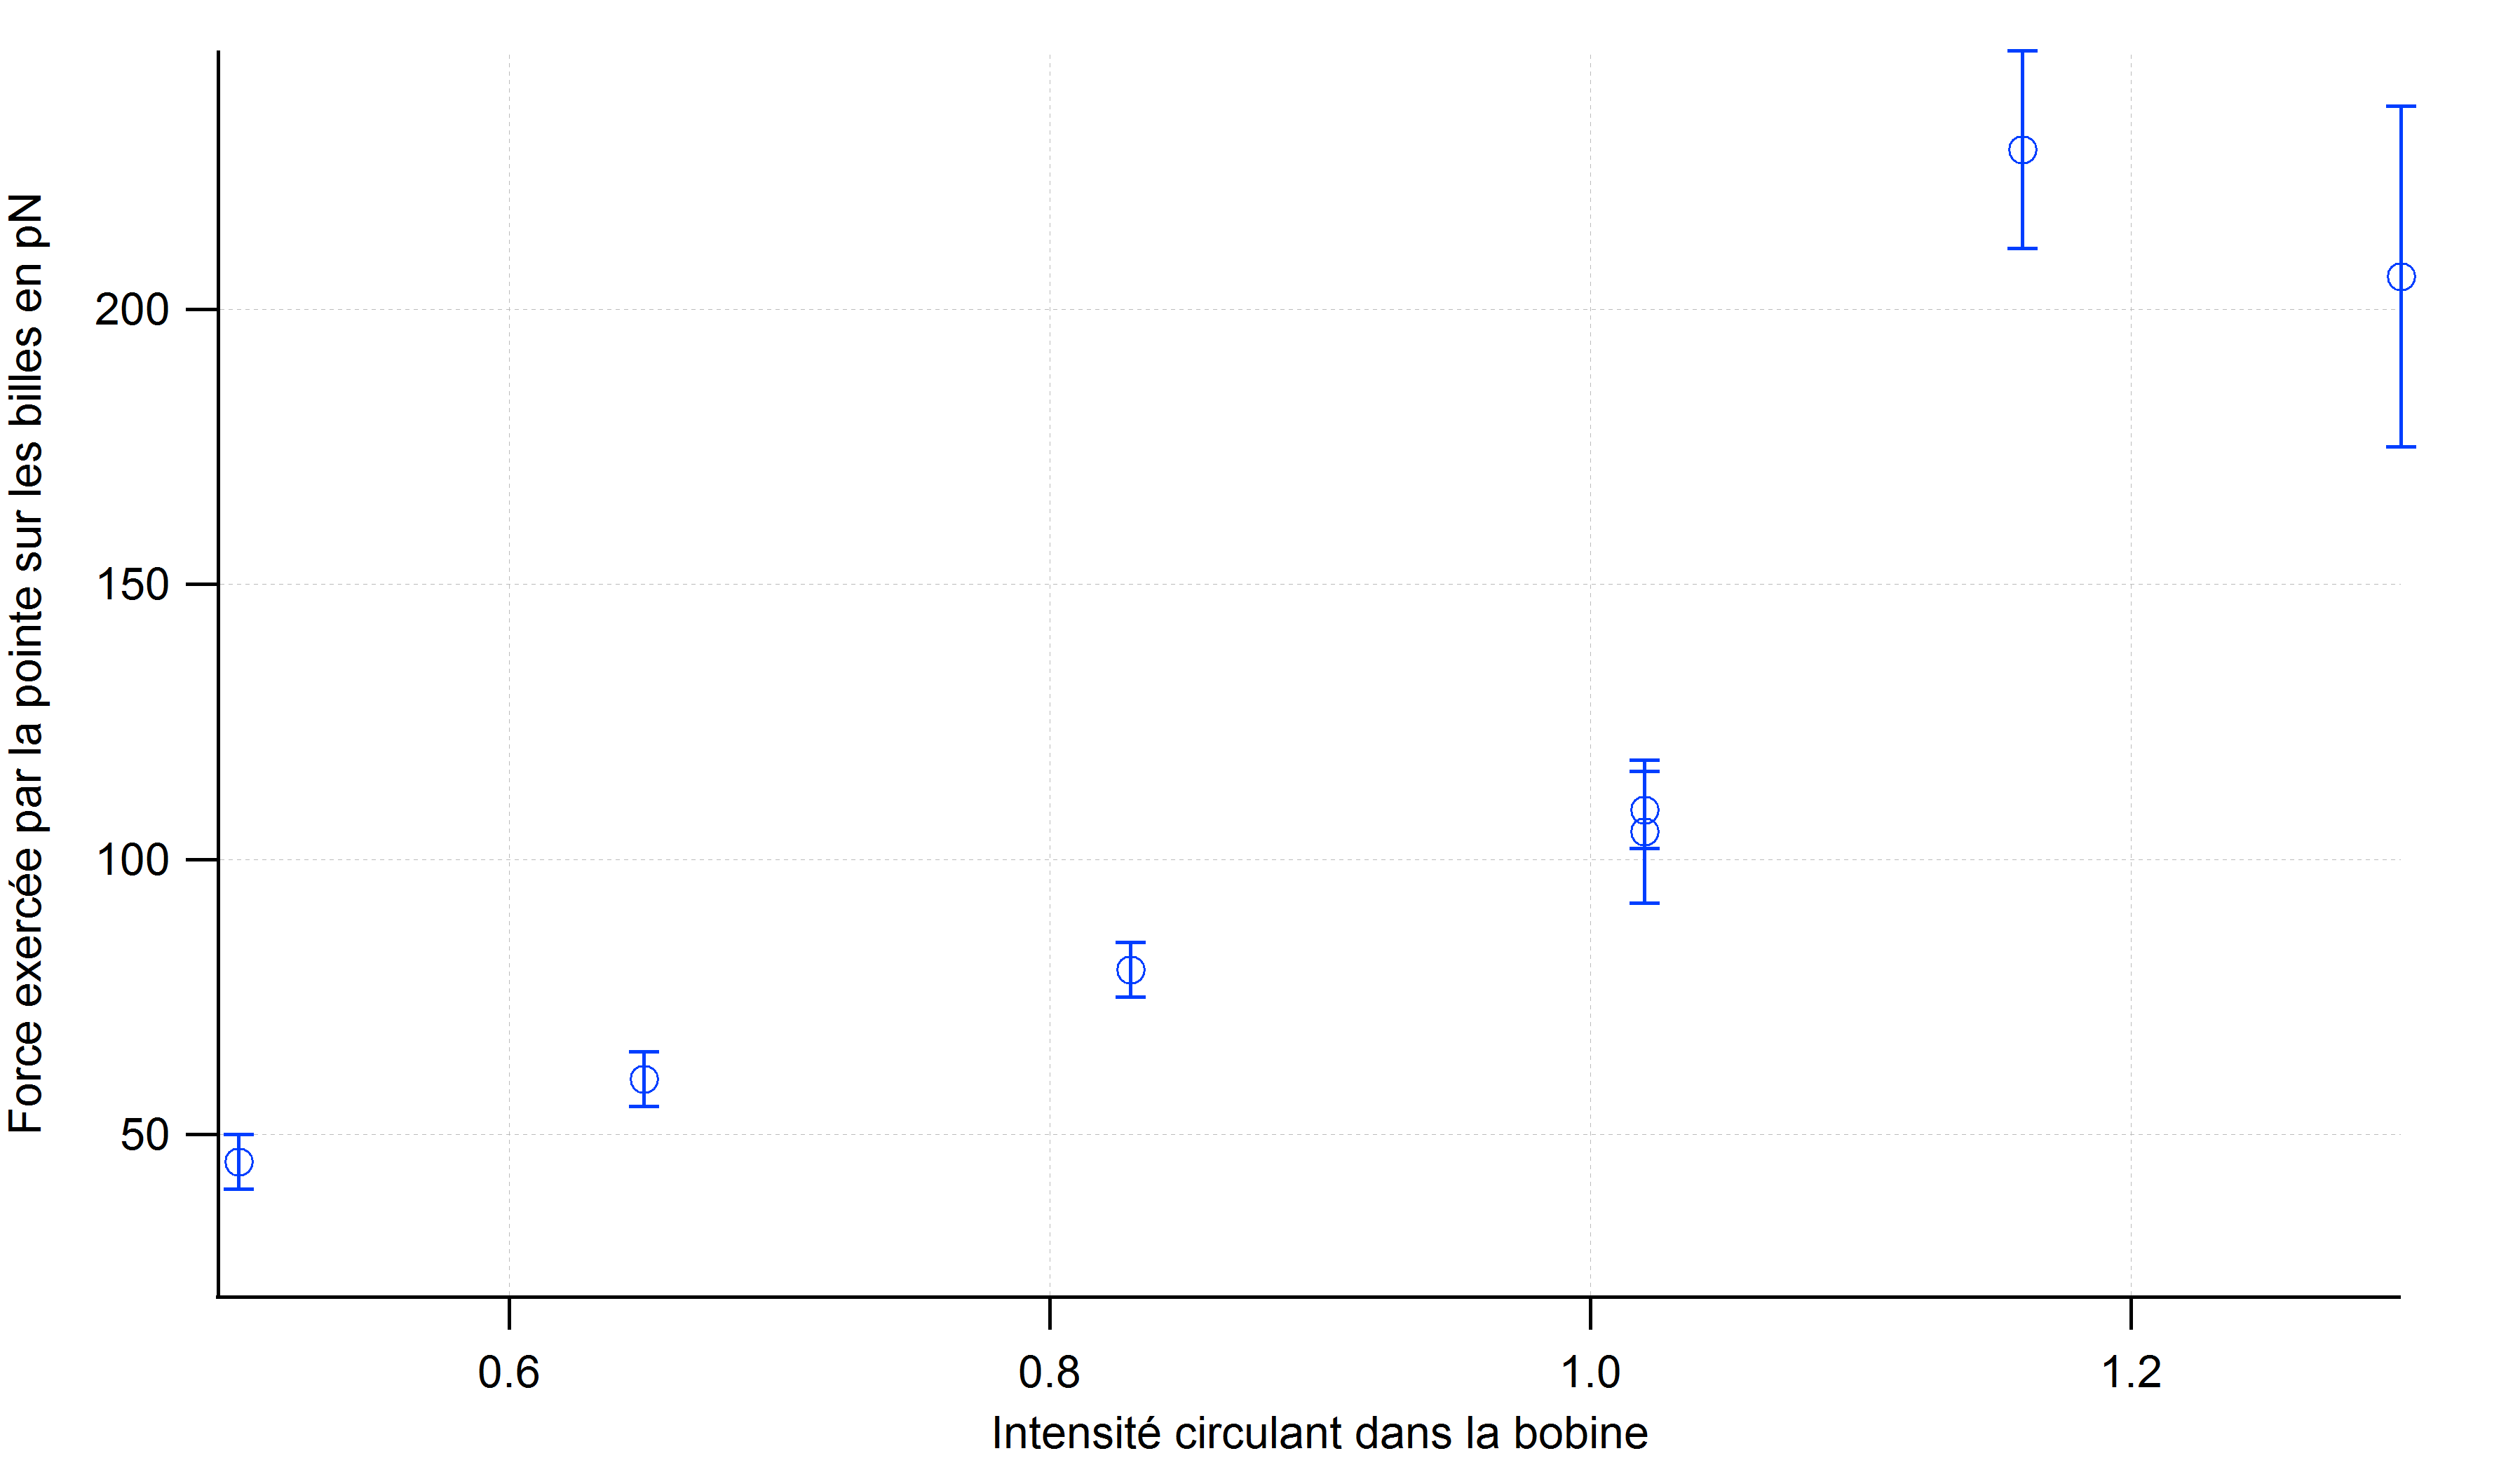
\includegraphics[scale=0.5]{Calibration_resume.png}
 \caption{Courbe de calibration des forces exercées à 700\micro m de la pointe. }
 \end{figure}
	
	
	\subsection{Protocole de mesures mécaniques}
	\subsubsection{Préparation des cellules et des billes}
	
	Les cellules sont ensemencées sur une lamelle de verre recouverte de fibronectine comme indiqué en \ref{Coating} 24 heures avant le début des expériences. 
	
	\paragraph{Ingrédients : }
	\begin{quote}
	Pour la fabrication de la suspension de billes fonctionnalisées : 
	\begin{itemize}
	\item PBS
	\item la suspension mère de Dynabeads à 4.10$^{8}$ billes/ml
	\item de l'eau micro-filtrée 
	\item un aimant permanent
	\item de la fibronectine
	\item une cuve à ultra-sons
	\end{itemize}
	Pour la préparation finale : 
	\begin{itemize}
	\item des C2C12 sur une lamelle de verre recouverte de fibronectine
	\item 50 \micro l de solution intermédiaire
	\item 950 \micro l de DMEM 1\% BSA
	\item du milieu complet
	\item une lamelle de verre 22mm*64mm*0.15mm
	\item un séparateur de 240\micro m d'épaisseur
	\item 15 \micro l d'HEPES
	\end{itemize}
	\end{quote}
	
	\paragraph{Protocole : }
	\begin{quote}
	\begin{enumerate}
	\item Suspendre 50 \micro l de suspension mère de Dynabeads dans 450  \micro l d'eau micro-filtrée. 
	\item Placer l'aimant sous l'eppendorf pour attirer les billes, et prélever 450 \micro l de surnageant.
	\item Suspendre à nouveau dans 450 \micro l d'eau.
	\item Répéter deux fois les deux étapes précédentes, mais la dernière fois, ajouter 450 \micro l de PBS au lieu de l'eau. 
	\item Placer l'eppendorf 15 minutes dans la cuve à ultra-sons pour disperser les billes, et vortexer toutes les 5 minutes.
	\item Ajouter 1 à 5 \micro l de fibronectine 1\micro g/ \micro l  dans la suspension
	\item Laisser incuber 30 minutes à 37 \degres C. 

La solution intermédiaire ainsi préparée peut être conservée à 4 \degres C pendant 4 à 6 semaines. 

Une heure avant la première expérience : 
	\item Placer l'eppendorf dans la cuve à ultra-sons pendant 15 à 30 minutes en agitant toutes les 5 minutes pour disperser à nouveau les billes
	\item Prélever 50 \micro l de suspension et les suspendre dans 950 \micro l de DMEM 1\% BSA. 
	\item Ajouter 75 \micro l de cette suspension sur une lamelle de C2C12.
	\item Laisser incuber les billes et les cellules ensemble pendant 30 minutes à 37 \degres C. 
	\item Rincer 2 fois avec 1ml de milieu en cisaillant le moins possible pour enlever les billes qui n'ont pas adhéré aux cellules. 
	\item Ajouter 15 \micro l d'HEPES pour tamponner le milieu pendant l'expérience.
	\item Coller le séparateur sur la lamelle 22mm*64mm*15mm lavée à l'alcool 70\%
	\item Ajouter 65\micro l de milieu 1,5\% d'HEPES
	\item Monter la lamelle de C2C12 pour fermer la chambre expérimentale.  
 
	\end{enumerate}
	\end{quote}
La lamelle préparée ainsi peut être observée immédiatement et conservée jusqu'à 2h dans une enceinte thermalisée à 37 \degres C. 	 	
	
	\subsubsection{Déroulement de l'expérience de fluage}
	
	On place la lamelle préparée à l'étape précédente sur le microscope inversé. 
	\paragraph{Protocole : }
	\begin{quote}
	\begin{enumerate}
	\item Au 20X, repérer la face supérieure de la lamelle au-dessus de la chambre expérimentale.
	\item Grâce au vernier de la tour à objectif, placer le plan focal 100 \micro m au-dessus de la lamelle. 
	\item Approcher la pointe avec le micromanipulateur afin de la placer dans le plan focal et au centre du champ de la caméra. 
	\item Décaler horizontalement vers la droite la pointe de 240 \micro m dans la configuration courte distance et de 390 \micro m dans la configuration longue distance. La pointe est alors alignée de sorte que l'axe de la bobine passe par le centre du champ d'observation. 
	\item Mémoriser cette position et éloigner la pointe.
	\item Décaler la lamelle, changer d'objectif pour le 100X en configuration longue distance, pour le 40X sinon.
	\item Placer une goutte d'huile sur l'objectif s'il s'agit du 100X et repositionner la lamelle. 
	\item Chercher une cellule sur laquelle a adhéré une bille unique et placer la bille au centre du champ d'observation.
	\item Ramener la pointe à la position mémorisée.
	\item Alimenter la pointe avec un signal sinusoïdal de fréquence 0.5Hz afin de chercher la plus petite intensité de courant pour laquelle la bille a un mouvement détectable. 
	\item Régler le GBF pour fournir la tension continue correspondante en réponse à un déclenchement externe (la carte PCI reliée à l'ordinateur). 
	\item Ajouter la lentille 1.5X dans l'axe optique.
	\item Sélectionner une zone restreinte autour de la bille qui va être acquise par la caméra.
	\item Lancer l'exécution du script sous MicroManager.
	\end{enumerate}
	\end{quote}
	
	Le script d'acquisition sous MicroManager contrôle la caméra et l'électro-aimant par l'intermédiaire de la carte PCI contrôlant le GBF. Il va procéder ainsi : 
	
	\begin{enumerate}
	\item[\textbf{Phase 1} : ]\textbf{de t=0 à t=12s}
	\item Déclencher l'acquisition d'images par la caméra en mode \emph{Burst}, c'est-à-dire aussi vite que possible. Cette vitesse est d'autant plus grande que la zone à observer est petite. 
	\item Déclencher le GBF pour allumer l'électro-aimant au courant pré-programmé sur le GBF. 
	\item[\textbf{Phase 2 :} ] \textbf{de t=12s à t=125s}
	\item Continuer l'acquisition des images de la bille mais à une vitesse réduite de 2 images/seconde.
	\item[\textbf{Phase 3 : }] \textbf{de t=125s à t=250s}
	\item Couper l'alimentation de l'électro-aimant
	\item Continuer l'acquisition à 1 image/seconde
	
	\end{enumerate}
	
	Cette séquence est répétée 4 ou 6 fois afin d'observer les différences de la fonction de fluage d'une expérience à la suivante. 
	
	 \`A la fin de l'expérience, nous obtenons une série d'images de la bille au cours du temps. 
	 Dans les métadonnées de ces images, il est possible d'obtenir l'heure à laquelle a été prise chaque image, ce qui permet d'avoir pour chaque image une coordonnée temporelle. 
	
	\subsection{Dépouillement des vidéos}
	
	Il est nécessaire d'analyser les images obtenues pour obtenir ce qui nous intéresse : la position de la bille au cours du temps. 
	
	Les premières images obtenues pour ma thèse ont toutes été traitées avec l'algorithme \emph{Analyse Particules} d'ImageJ. 

Par la suite, pour les expériences menées plus tardivement avec Pierre-Olivier Strale, nous avons préféré utiliser Icy et son plugin \emph{Active Contours}, qui est beaucoup plus robuste à une défocalisation de la bille. 

	Le traitement d'image nous fournit la position de la bille, le grand axe et le petit axe de la bille et la distance au centre du noyau en fonction du temps écoulé depuis le début de l'application de la force. 
	
	
	\begin{figure}
	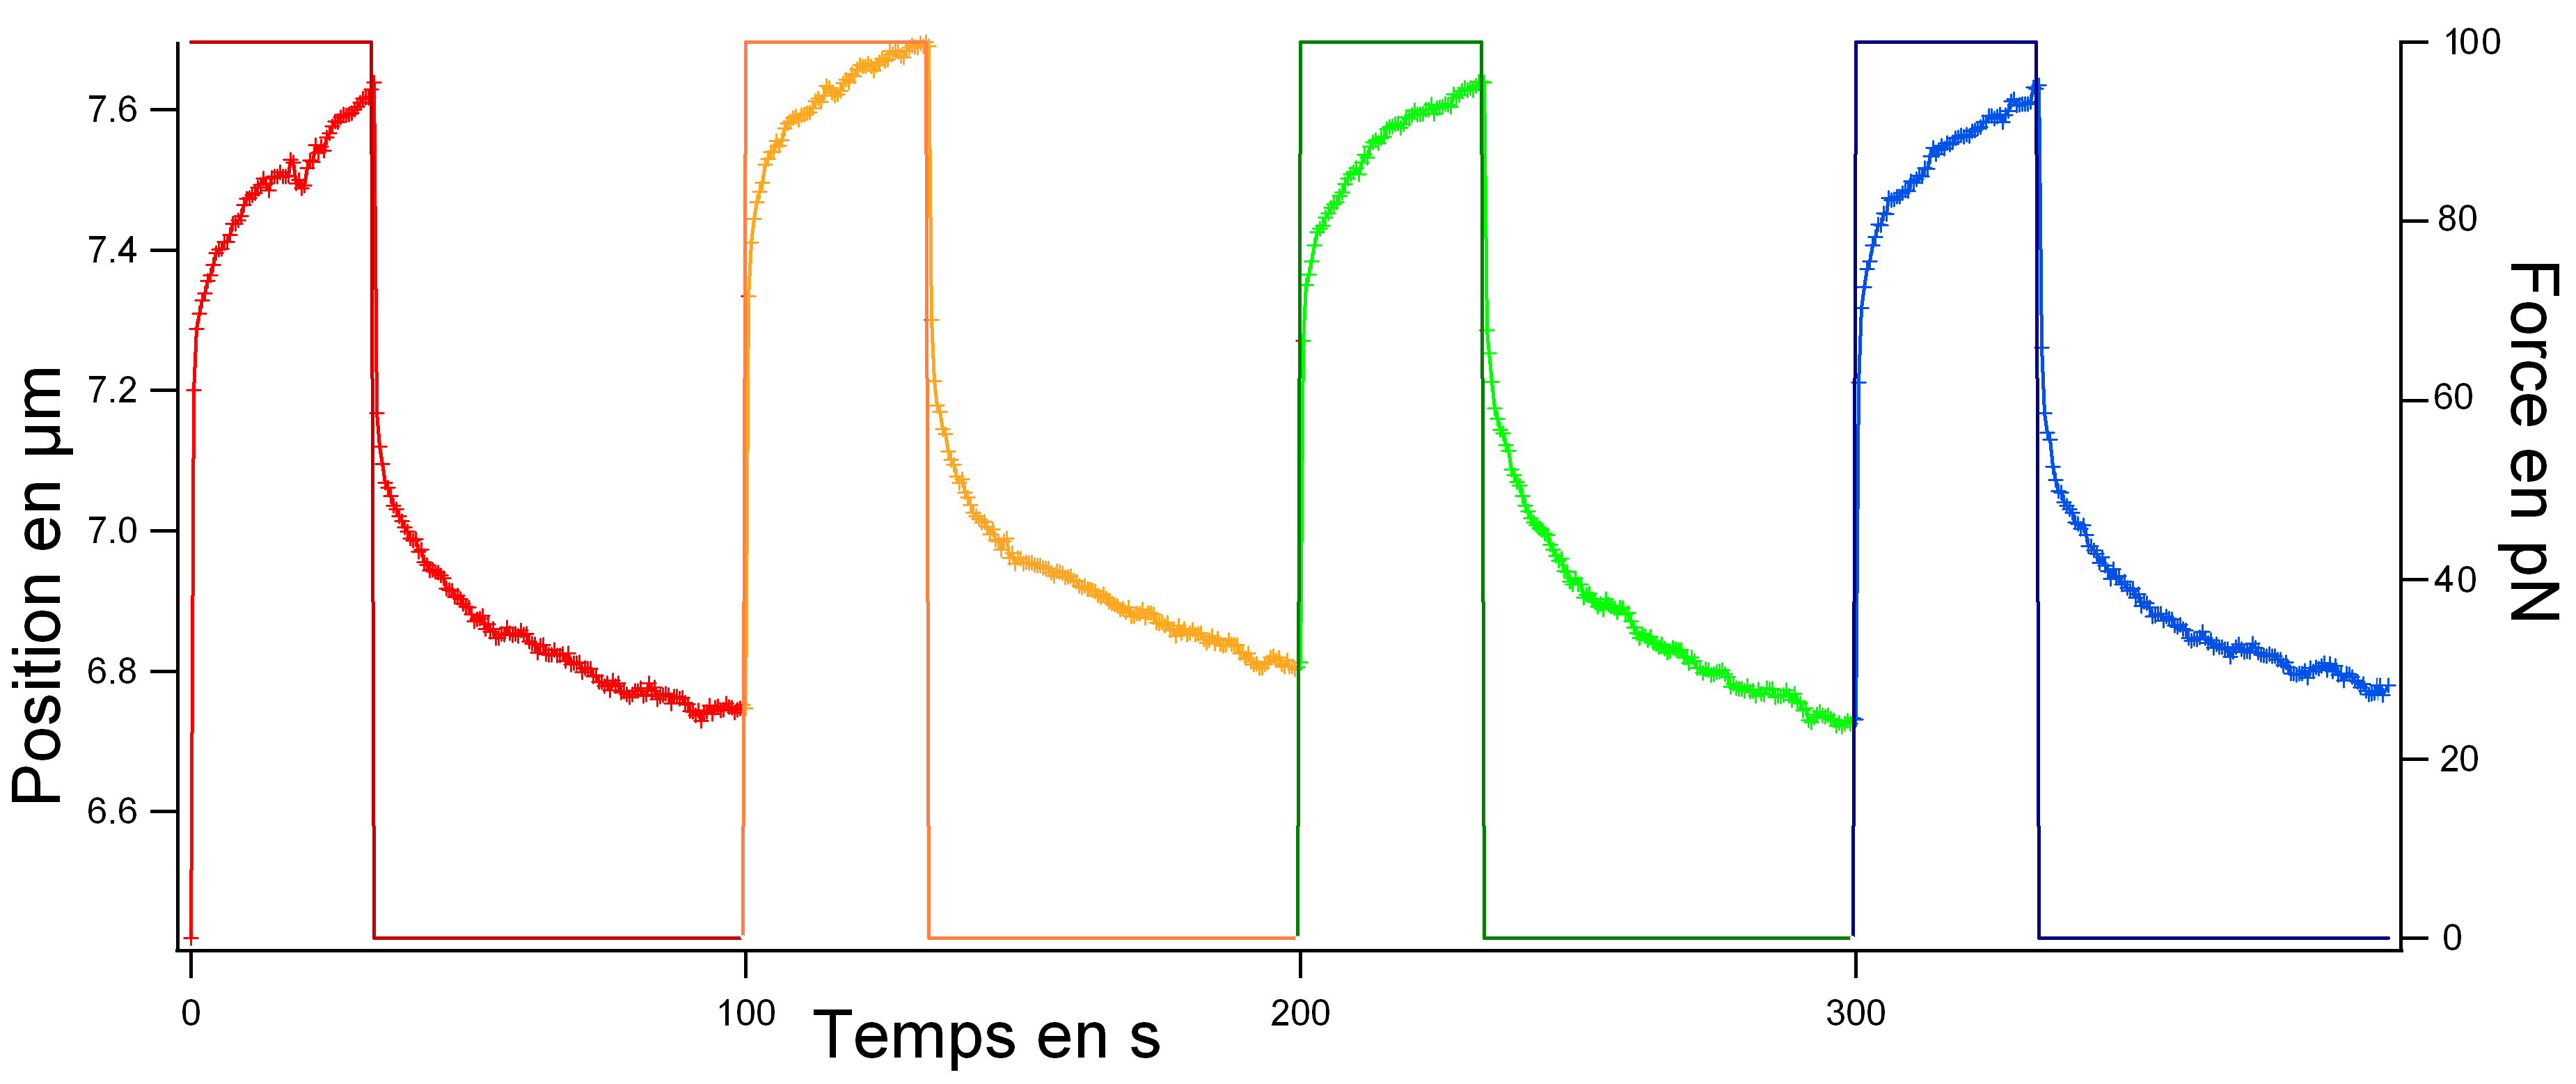
\includegraphics[scale=0.11]{c9-rigidification-couleurs.png}
	\caption{Déplacement au cours du temps d'une bille adhérant sur une C2C12 et soumise à 4 créneaux de force de 100pN pendant 33s toutes les 100s. }
	\end{figure}
	\subsection{Fonction de fluage}
	\`A l'issue d'une expérience, nous obtenons donc la position de la bille au cours du temps, en fonction de la force appliquée, pour 4 à 6 applications de la force. 
	
	Cependant, pour obtenir des mesures de modules visco-élastiques, il est nécessaire d'utiliser un modèle reliant le mouvement de la bille à la déformation de la cellule, et la force exercée sur la bille à la contrainte subie par la cellule.
	Plusieurs modèles existent, en particulier un modèle théorique, le modèle de Gallet, et un modèle numérique développé dans la thèse d'Alain Kamgoué, mais les deux supposent que la bille est soumise à une force incluse dans le plan focal du microscope, ce qui n'est pas le cas de notre pince magnétique, qui tire également verticalement. 
	
	Le modèle de Gallet suppose que la bille est enfoncée d'un angle $\theta$ dans la cellule, et qu'elle est soumise à une force horizontale $\vec{F}_0$. La cellule est modélisée comme un milieu visco-élastique semi-infini homogène et isotrope. La bille est supposée s'ancrer dans la cellule de manière homogène et infiniment rigide. 
	La valeur de la fonction de fluage est alors donnée par : 
	\begin{equation}
	J(t)=2\pi a \frac{2}{3}\left(\frac{1}{\left( \frac{3}{2 \sin \theta}+\frac{\cos \theta}{\sin^3 \theta}\right)} \right)  \frac{\delta R(t)}{F_0} 
	\label{Fluage}
	\end{equation}
	où $a$ est le rayon de la sphère, $\theta$ l'angle d'enfoncement dans le milieu visco-élastique, $\delta R$ le déplacement de la bille et $F_0$ la composante horizontale de la force exercée sur la bille. 
	
	Passons en revue les différentes approximations.
	
	 L'ancrage de la bille à la cellule est assurée par les liaisons fibronectine-intégrine ponctuellement sur la surface de bille immergée dans la cellule. Il nous est impossible avec les techniques dont nous disposons d'avoir une quelconque idée de la quantité de liaisons ponctuelles à la surface de contact. Cependant, en plus des contacts spécifiques, la cellule peut établir avec la membrane des contacts non spécifiques. La supposition d'un très grand nombre de sites de liaisons au niveau de la surface de contact est donc crédible. On l'a vu précédemment, au niveau du complexe d'adhésions à l'intérieur de la cellule, la situation est extraordinairement complexe. Lorsque l'on sonde par les intégrines, on sonde la rigidité de l'ensemble de l'assemblage complexe qui les relie au cytosquelette d'actine. 
	
	La cellule est considérée comme un milieu semi-infini. 
	Cette approximation serait facile à justifier si la bille était de taille négligeable par rapport à l'épaisseur de la cellule, mais l'épaisseur de la cellule et la taille de la bille sont en fait presque égales; et souvent, la bille est plus grande que l'épaisseur de la cellule lorsqu'elle est loin du noyau. 
	Cependant, la cellule n'est certainement pas non plus isotrope. 
	En effet, lorsqu'avec les pinces magnétiques, on exerce une force ayant deux composantes égales, l'une horizontale et l'autre verticale, la bille n'a un mouvement détectable que dans le plan horizontal. 
	Dans le plan vertical, la bille ne sort pas du plan focal, alors qu'un mouvement très faible serait immédiatement détectable par l'intermédiaire des anneaux de diffraction. 
	Sur le verre, les C2C12 sont très étalées et leur surface inférieure est ancrée à la fibronectine adsorbée sur le verre de façon très forte et la rigidité des cellules selon l'axe vertical est beaucoup plus grande à la fois que la rigidité dans les deux autres directions, mais aussi que la gamme de ridigités que nous pouvons sonder avec les pinces magnétiques. 
	
	Enfin, la cellule est considérée comme un matériau passif, ce qui n'est le cas que pendant les 10 à 20 premières secondes d'application de la force. 
	Après ce temps, il devient évident que la cellule exerce activement des forces sur la bille. 
	C'est pourquoi il faut se limiter à appliquer ce modèle pendant les premières 10 secondes de l'application de la force, et c'est pour cette raison qu'il est important de prendre le plus d'images possible pendant ce temps. 
	
	Durant sa thèse sous la direction de Jacques Ohayon, Alain Kamgoué a développé un modèle à partir de simulations numériques, qui prend à en compte à la fois l'angle d'enfoncement de la cellule et l'épaisseur finie de la cellule sous la bille, mais qui considère alors la cellule comme un matériau purement élastique dont il cherche à extraire le module d'Young. Il calcule alors un préfacteur géométrique : 
$$ p(\theta,\frac{h_u}{2R})=\frac{ F_0}{2 \pi a \delta R(t) E} $$

avec $h_u$ la hauteur de la cellule sous la bille, et $E$ le module d'Young de la cellule. Ce qui nous donne, en le mettant sous la même forme que l'équation \ref{Fluage} : 
\begin{equation}
J= 2 \pi a p(\theta,\frac{h_u}{2R}) \frac{\delta R(t)}{F_0}
\label{Kamgoué}
\end{equation} 

La différence entre les deux modèles est donc uniquement le facteur géométrique, qui dépend dans les deux cas de l'enfoncement de la bille, et dans le second cas également de l'épaisseur de la cellule en-dessous de la bille.

Durant les expériences de pinces magnétiques, nous ne pouvons pas mesurer l'angle d'enfoncement des billes. Cependant, des cellules fixées ont été observées au microscope confocal, ce qui nous a permis de mesurer l'angle d'enfoncement des billes, et la hauteur $h_u$ pour 23 billes. On obtient alors : 
$$ \langle h_u \rangle = 1.6 \mu m \: \langle \theta \rangle = 110 \degres$$

Ce qui nous donne avec les deux modèles : 
\begin{align}
 p_{Gallet}&=\frac{2}{3}\left(\frac{1}{\left( \frac{3}{2 \sin \theta}+\frac{\cos \theta}{\sin^3 \theta}\right)} \right) = 0.50 \\
p_{Kamgoue}&= 0.92\\
\end{align}

Les deux modèles donnent donc deux valeurs différentes, mais ayant le même ordre de grandeur. 
Les deux supposent une force horizontale, ce qui est faux ici. Le modèle de Gallet prend en compte le caractère visco-élastique de la cellule, mais en faisant l'hypothèse d'un milieu semi-infini, alors que le modèle de Kamgoué-Ohayon considère une épaisseur finie mais oublie la composante visqueuse du milieu cellulaire. 

Le véritable préfacteur se trouve probablement entre les deux, et en réalité ce n'est pas l'essentiel ici : il s'agit d'observer l'évolution des paramètres mécaniques de la cellule au cours du temps, et cette comparaison reste strictement identique quel que soit le préfacteur utilisé. 
C'est pourquoi les résultats seront en général présentés uniquement sous la forme $\frac{\delta R(t)}{F_0}$ sans tenir compte du préfacteur géométrique. 




	
	
\section{\'Etirement}
	L'objectif de ce dispositif est de soumettre les cellules à une déformation constante pendant plusieurs heures et de les observer en fluorescence pendant l'étirement sur un microscope inversé. 
	
	Les expériences de pinces magnétiques ont l'avantage de nous renseigner quantitativement sur les paramètres rhéologiques de la cellule. Cependant, elles nous obligent à une observation cellule par cellule, ce qui rend la construction d'une étude statistique très longue. Avec l'étireur on peut observer une trentaine de cellules simultanément pendant deux heures, alors qu'avec les pinces magnétiques on aurait pendant ce temps observé 4 cellules pendant 30 minutes chacune.
	
	\subsection{Description de l'étireur}
	Pendant ma thèse j'ai conçu les plans de cet étireur de cellules qui a ensuite été réalisé par l'atelier du laboratoire. Il est composé de trois parties principales : la cuve, le support de lamelle et le plot. Toutes les parties de l'étireur sont en PVC, sauf le plot qui est en plexiglas transparent pour laisser passer la lumière du condenseur. L'étireur à une symétrie cylindrique autour d'un axe vertical. 
	\begin{figure}
	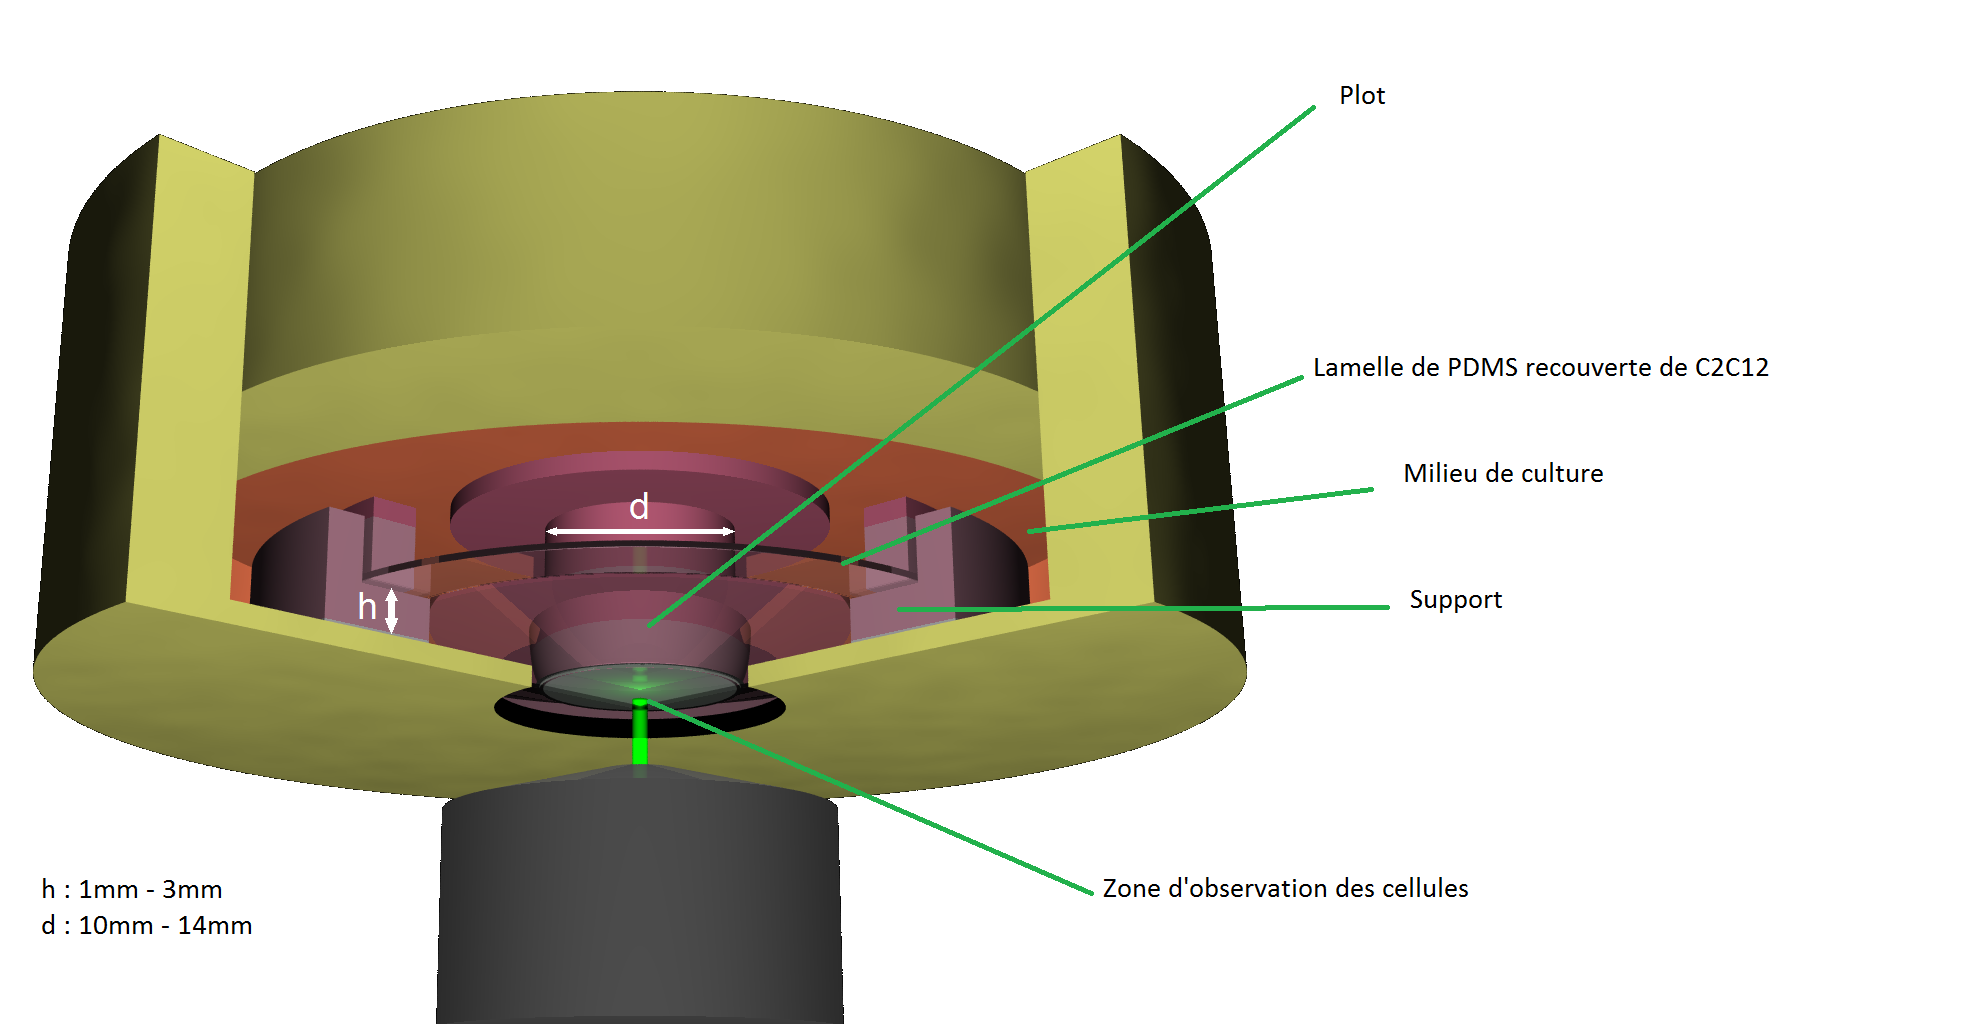
\includegraphics[scale=0.2]{Etireur_3D_vue_dessous_rayon_blanc.png}
	\caption{Modélisation de l'étireur vu de dessous pendant l'étirement.}
	\end{figure}
	\subsubsection{La cuve}
	La cuve doit remplir deux fonctions : contenir le milieu de culture nécessaire aux cellules et permettre l'observation de celles-ci au microscope inversé. Elle est composée de deux pièces trouées en leur centre qui se vissent l'une dans l'autre. Au niveau de l'ouverture destinée à l'observation, on place une lamelle de verre de 30 mm de diamètre dont le contour a été préalablement enrobé dans du téflon souple. Cette lamelle de verre est enserrée entre les deux pièces de façon à former une cuve étanche dont le fond transparent permet l'observation.
	\subsubsection{La lamelle de PDMS} 
	Les cellules adhèrent à une lamelle de PDMS réticulé élastique recouverte de fibronectine. Cette lamelle est maintenue par le support et déformée par le plot qui la pousse vers le bas. 
	Le PDMS (Sylbard Silicon Elastomer, Dow Corning) est fabriqué à partir d'un mélange 90\% PDMS et 10\% de réticulant. On place alors 1,8g du mélange dans une boite de Petri de 90 mm de diamètre et on l'étale par drainage jusqu'à la recouvrir entièrement de manière homogène. La masse est choisie de façon à ce que le PDMS étalé fasse 0,3mm d'épaisseur. Les boîtes recouvertes de PDMS sont alors placées toute la nuit dans un incubateur à 60\degres  C pour réticuler l'élastomère. À l'aide d'un emporte-pièce, des disques de 30mm sont alors découpés dans les boîtes.

		
	\subsubsection{Le support}
	Le support est la pièce de serrage de la lamelle de PDMS sur laquelle sont cultivées les cellules. La lamelle de PDMS est placée entre deux anneaux plats de téflon d'un millimètre d'épaisseur qui sont destinés à homogénéiser la pression exercée sur la lamelle par la pièce de serrage. L'ensemble est posé sur un support de hauteur 1 mm ou 3mm qui va déterminer l'étirement maximal possible, et serré par une pièce qui se visse dans le support. 
	Cette pièce doit maintenir fermement les bords de la lamelle en place tandis que le centre est étiré par le plot. 
	\subsubsection{Le plot}
	Le plot transparent est maintenu dans une pièce qui se visse à l'intérieur de la cuve. Le vissage va faire descendre le plot, qui va ainsi étirer la lamelle en la rapprochant du fond de la cuve et donc de l'objectif du microscope. Le pas de vis fin fait descendre de 1mm la membrane à chaque tour. 
	L'utilisation du support de 1mm ou de 3mm permet de fixer la lamelle de PDMS à différentes hauteurs, et donc pour un même abaissement du plot d'étirer plus ou moins la lamelle. Il existe deux diamètre de plots cylindriques : 10mm et 14mm, qui permettent également de régler l'étirement subi par le PDMS. 
	\subsection{Calibration de l'étireur}
	
	Un modèle géométrique simple permet d'estimer rapidement l'augmentation de la surface de la lamelle de PDMS en fonction du diamètre et de l'enfoncement du plot : 
	$$R_{etire}=R_p+\sqrt{h^2+(R_l-R_p)^2}$$
	$$ \frac{\Delta A}{A} = \frac{R_{etire}^2}{R_l^2}-1$$ 	
		
	\begin{figure}[h!]
		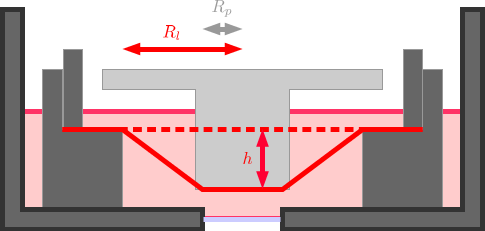
\includegraphics[scale=0.5]{Modele_etireur.png}
		\caption{Modèle simple de la déformation créée par l'étireur. $R_p$ est le rayon du plot, $R_l$ le rayon de la lamelle qui n'est pas maintenu par le support et $h$ la hauteur d'enfoncement du plot.}
		\end{figure}	
		
		\begin{figure}
		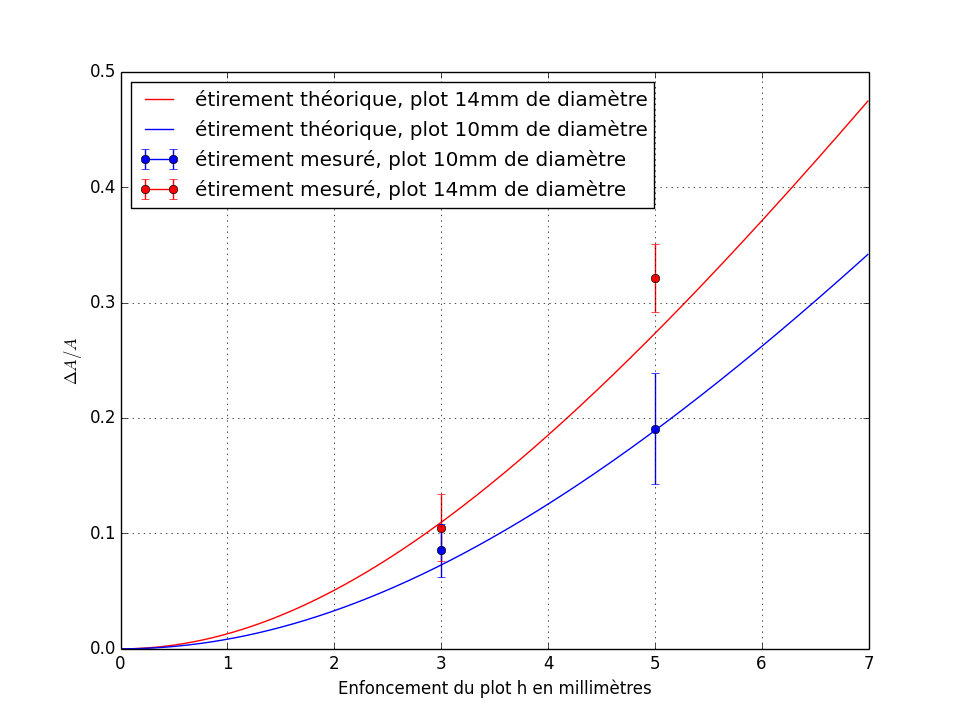
\includegraphics[scale=0.5]{Figures/Calibration_etireur.png} 
		\caption{Résultats de la calibration de l'étireur pour les différents étirements utilisés comparés au modèle théorique, pour $R_p$= 5 ou 7 mm et $R_l$=13mm}
		\end{figure}
	Afin de le comparer à l'étirement réel subi par la lamelle de PDMS, des lamelles ont été recouvertes de Pluronic (Pluronic F-127, Sigma Aldrich), un copolymère photosensible, puis exposées à un rayonnement UVC afin d'oxyder le Pluronic à travers un masque de quartz imprimé d'une fine couche de métal formant un grand nombre de carrés de taille connue formant un quadrillage. Puis les lamelles ont été recouvertes de fibronectine fluorescente, qui ne pouvait adhérer qu'aux endroits non éclairés par les UV. 
	
	\paragraph{Ingrédients : }
	\begin{itemize}
	\item une lamelle de PDMS vierge
	\item Pluronic
	\item Fibronectine Cy3
	\item un masque en quartz 
	\item une lampe UVC
	\end{itemize}
	
	\paragraph{Protocole}
	\begin{enumerate}
	\item Préparer une solution de Pluronic 0,2\% en masse
	\item Laisser incuber 1 ml de la solution de Pluronic pendant une heure à température ambiante
	\item Rincer au PBS, puis à l'eau, laisser sécher
	\item Exposer la lamelle derrière le masque aux UVC pendant 7 minutes
	\item Diluer 4 \micro g de fibronectine fluorescente dans 1 ml de PBS
	\item Laisser la solution de fibronectine incuber 30 minutes à 37 \degres C sur la lamelle, à l'abri de la lumière
	\item Rincer au PBS et stocker à 4 \degres C dans le PBS, à l'abri de la lumière
\end{enumerate}		
	
	Nous avons ainsi obtenu des lamelles recouvertes d'un quadrillage visible en microscopie de fluorescence. Ce quadrillage a été observé avant et après étirement, et l'étirement a alors été mesuré à partir de la formation du quadrillage.
	
%	\begin{figure}
%	\includegraphics[scale=0.05]{Calibration_plot.png}
%	\includegraphics[scale=0.05]{Calibration_fibro_(RGB).png}
%	\caption{À gauche : image du plot reconstituée à partir d'images prises au 4X sur le microscope confocal. À droite : images en fluorescence du quadrillage de fibronectine Cy3 avant (en rouge) et après (en bleu) un étirement 30\%.}
%	\end{figure}
	
\begin{figure}
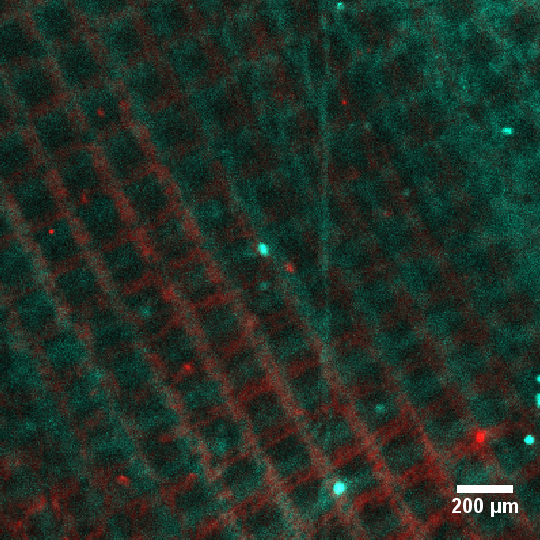
\includegraphics[scale=0.3]{Figures/Zoom_Calibration_etireur.png} 

\caption{Superposition des images prises en microscopie de fluorescence du quadrillage de fibronectine Cy3 imprimé sur une lamelle de PDMS avant(en rouge) et après (en bleu) étirement. }
\end{figure}
	Les images nous montrent que la déformation du PDMS par le plot est radiale et uniforme, et que le modèle géométrique le plus simple décrit bien quantitativement la déformation subie. 
	
	\subsection{Le microscope confocal}
	
	Pour les expériences d'étirement, nous avons utilisé le microscope confocal du laboratoire car il dispose d'une platine motorisée, de 4 lasers et des filtres automatisés. Cependant, l'étireur impose d'avoir un plan focal situé à une grande distance de l'objectif, ce qui impose l'utilisation d'un objectif à air à grande distance de travail. Cela nous interdit malheureusement de profiter de la fonctionnalité du confocal qui est de faire des images en 3D. 
	
	Les observations en fluorescence contiennent donc nécessairement une intégration du signal selon l'axe vertical, ce qui implique que les endroits où la cellule est épaisse apparaissent comme plus lumineux que les endroits où elle est fine. 
	
%	Il en ressort que la zone du noyau, la plus épaisse de la cellule, est presque toujours plus lumineuse que les bords de la cellules qui sont très fins. 
%	Il peut alors se révéler peu pertinent de comparer la fluorescence du cytoplasme en entier et la fluorescence du noyau lorsqu'on veut comparer la concentration d'une protéine fluorescente de part et d'autre de la membrane nucléaire.
%	
%	C'est pourquoi il peut être intéressant de regarder non seulement toute la cellule, mais également une zone péri-nucléaire, d'épaisseur comparable à celle du noyau. Entre le noyau et la zone péri-nucléaire, on compare des luminosités à épaisseur fixée.
	
	\paragraph{Description générale}
	
	Le microscope confocal est un modèle \og spinning  disk \fg d'Andor, composé : 
	\begin{itemize}
	\item d'un microscope inversé Olympus IX81
	\item de 4 lasers Andor Laser Combiner 400 series et des AOTF qui permettent de couper une partie de leur puissance.
	\item d'une roue motorisée de 10 filtres Sutter Lambda 10B Controller
	\item d'un disque rotatif Yokogawa CSUX1
	\item d'une platine motorisée Prior Proscan II
	\item d'un platine piézo de réglage pour l'axe Z Andor APZ-100
	\item d'une caméra EMCCD IXON+ Andor Technologies
	\item d'un ordinateur avec le logiciel constructeur IQ2 pour contrôler l'ensemble
	\item d'une enceinte thermalisée par un Cube 2 de Life Imaging Services
\end{itemize}	 

Dans les expériences décrites, sauf indications contraires, il sera utilisé avec un objectif 20X à air Olympus à grande distance de travail (Olympus LUCPLFLN 20X, ouverture numérique 0.45, distance de travail 6.6 - 7.8 mm).

Quatre configurations d'observation ont été utilisées pour la fluorescence : 
\begin{itemize}
\item[Rouge profond] : Laser d'excitation 640nm et filtre 685nm
\item[Rouge] : Laser d'excitation 561nm et filtre 607nm
\item[Vert] : Laser d'excitation 488nm et filtre 525nm
\item[Bleu] : Laser d'excitation 405nm et filtre 465nm
\end{itemize}
	
	\subsection{Protocole d'étirement observé en direct}
	Les cellules sont ensemencées sur des lamelles de PDMS préalablement recouvertes de fibronectine. Afin d'améliorer l'efficacité de transfection, dans le protocole final, les cellules sont transfectées avec la nanofectine pendant 6h avant d'être rincées décollées, comptées et ensemencées à raison de \nombre{110000} cellules par lamelle. 
	
	Après avoir mené un certain nombre d'expériences, nous avons constaté que la sensibilité de MRTF-A à la stimulation par le sérum est telle que le fait de remplacer le milieu de culture dans lequel les cellules baignaient depuis 24h par du milieu de culture neuf provoque des modifications non négligeables de la localisation de MRTF-A dans les cellules. Il est donc essentiel de conserver le même milieu de culture tout au long de l'expérience. 
	
	Après ensemencement et adhésion, les lamelles de PDMS peuvent être montées à l'avance sur le support et maintenues dans 5 à 7ml de milieu de culture blanc (5ml pour l'étirement 10\% et 7ml pour 30\%). 
	
	Juste avant l'expérience, la lamelle et le milieu de culture sont montés dans le reste de l'étireur et 1,5\% d'HEPES sont alors ajoutés pour tamponner le milieu pendant la durée de l'expérience. L'étireur complet est alors placé sur la platine du microscope et observé à l'aide d'un objectif 20X (trouver les caracs de l'objectif). Les cellules sont observées en lumière blanche et en fluorescence une première fois avant étirement brièvement, afin d'avoir une idée de l'état de départ des cellules. 
	
	En vissant le plot, on étire alors la lamelle rapidement en quelques secondes jusqu'à la déformation souhaitée. On cherche alors des cellules exprimant la MRTF-A GFP. À chaque fois qu'une ou plusieurs cellules sont visibles dans un champ, on enregistre la position de la platine motorisée. Toutes les 5 à 10 minutes, on retourne observer toutes les cellules répertoriées afin de suivre l'évolution de la localisation de MRTF-A au cours du temps. De nouvelles cellules sont recherchées jusqu'à 40 minutes après l'étirement et l'observation est ensuite maintenue pendant 2h après l'étirement. 
	\begin{figure}
	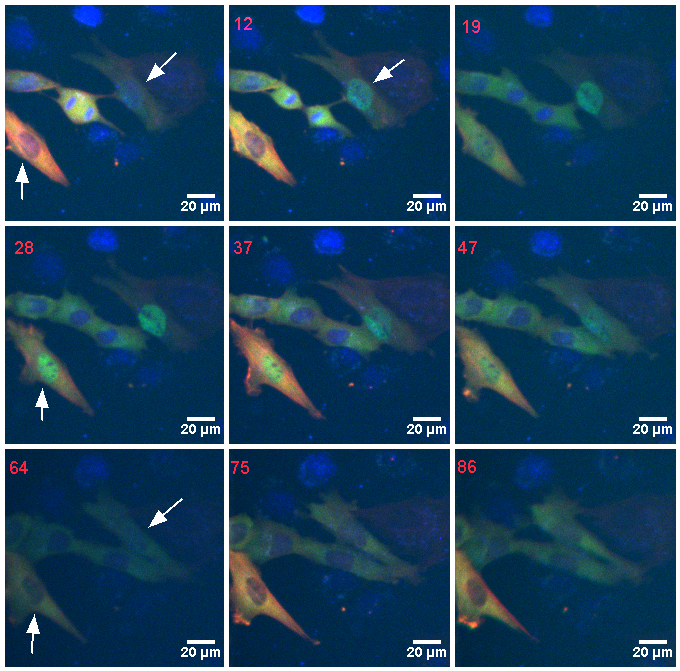
\includegraphics[scale=0.5]{Montage_translocations_2013-04-16_l2z1.png}
	\caption{C2C12 transfectées MRTF-A GFP (en vert) et Actine Mcherry (en rouge), marquées au DAPI (en bleu), étirées à 30\% pendant 120 minutes. Dans les deux cellules marquées d'une flèche, MRTF-A s'accumule dans le noyau, puis retourne dans le cytoplasme.}
	\label{Etirement_live}
	\end{figure}
	
	
	\subsection{Protocole d'étirement fixé}
	
	Le protocole d'étirement avec observation en direct ne nous permet pas d'observer la population de cellules à des instants courts, car il faut du temps pour retrouver un nombre suffisant de cellules. De plus, l'observation de l'état du cytosquelette en direct est difficile car les différents marqueurs disponibles perturbent trop le système : la sur-expression d'actine lors de la transfection avec une actine mCherry modifie de manière très visible l'équilibre entre MRTF-A et l'actine G, ce qui sera présenté au chapitre 8, la LifeAct RFP, qui marque les filaments d'actine, est exprimée tellement intensément que sa fluorescence empiète sur celle de MRTF-A GFP. La différence d'expression des deux plasmides peut être en partie due à la différence de poids moléculaire des deux protéines : MRTF-A est une grosse protéine d'environ 150 kDa, alors que la Life ne fait que 17 acides aminés de long. De plus, il n'existe pour l'instant aucun marqueur commercial permettant de visualiser l'actine G dans les cellules vivantes. 
	
	Fixer les cellules nous permet d'avoir un marquage quadrichrome : la F-actine en rouge-profond grâce à la phalloïdine Alexa 647, la G-actine en rouge grâce à la DNaseI Alexa 594, MRTF-A GFP ou anticorps anti-MRTF-A en vert et l'ADN du noyau en bleu grâce au DAPI. 
	
	\begin{figure}
	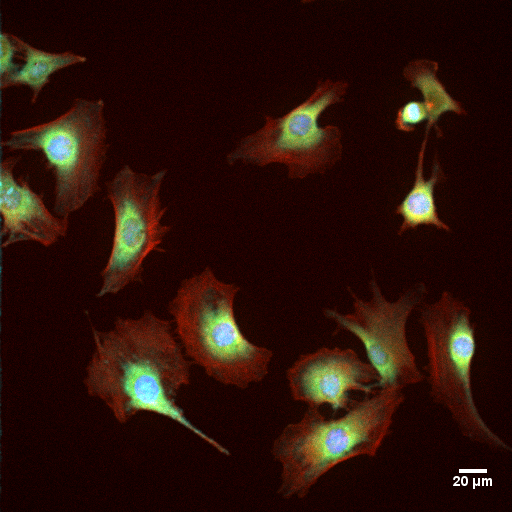
\includegraphics[scale=0.3]{2014-06-18-Et10-0-1(RGB).png}
	\caption{C2C12 marquées par la phalloïdine (ici en rouge), par la DNase I (en vert), un anticorps anti-MRTF-A (en cyan) et le DAPI (en bleu).}
	\end{figure}
	
	Pour une expérience d'étirement fixé, on prépare une boîte de C2C12 proches de la confluence (60-70\%) transfectées si l'on veut observer la MRTF-A GFP. Elles sont ensemencées ensemble sur 6 lamelles de PDMS dans une plaque 6 puits dans 3ml de milieu de culture 24h avant le début de l'expérience. Le lendemain, une de ces lamelles est montée sur le support, rincée au PBS et fixée immédiatement, c'est la lamelle témoin. Les autres lamelles sont successivement étirées, laissées à l'incubateur pendant un temps donné, puis démontées, rincées et fixées immédiatement. On obtient ainsi pour un même étirement une lamelle à t=0 et 5 lamelles à différents temps après étirement (par exemple 5, 10, 20, 30, 60 minutes après étirement). 
	
	Ces lamelles sont ensuite marquées dans les 4 couleurs suivant un protocole strictement identique, et observées avec des paramètres strictement identiques (intensité du laser, temps d'exposition \dots) au microscope, afin de pouvoir comparer quantitativement les intensité de fluorescence d'une lamelle par rapport aux autres. 
	

	\subsection{Dépouillement des images}
	\subsubsection{\'Etirement observé en direct, traitement qualitatif}
	On obtient après une observation en direct d'étirement typique une vingtaine de série d'images de cellules observées pendant 120 minutes après étirement, comme la série exposée en figure \ref{Etirement_live} le présente.
	Les images sont observées grâce à ImageJ, qui nous permet de reconstituer une pile d'images en 4 dimensions (x,y,temps et couleur). On peut alors observer qualitativement à l'\oe il s'il y a plus de MRTF-A GFP dans le noyau, dans le cytoplasme, ou si la répartition est homogène. 
	
	Toutes les données finales sont destinées à être stockées dans une base de données SQL. Cette forme de stockage de données permet de sélectionner et de trier les données en fonction de nombreux critères à la fois quantitatifs et qualitatifs. Pour remplir et interroger la base de données, j'ai également créé une interface en Python. Cette interface récupère dans les métadonnées des images prises au microscope les temps auxquels ces images ont été prises. L'utilisateur peut alors remplir pour chaque temps la localisation principale de MRTF-A dans la cellule : Nucléaire, Homogène ou Cytoplasmique. 
	Pour chaque champ d'observation, il note également le nombre de cellules visibles dans le champ, ce qui permet d'évaluer la densité locale de cellules. 
	
	Dans cette base de données, on retrouve alors pour chaque cellule la localisation de MRTF-A au cours du temps écoulé depuis l'étirement, l'étirement, le passage, le nombre de cellules présentes dans chaque champ, et l'expression en actine mCherry.
	\subsubsection{\'Etirement fixé, traitement quantitatif}	
	
	Pour chaque lamelle fixée, on obtient une série d'images en 5 couleurs : rouge profond, rouge, vert, bleu et lumière blanche. 

À partir des images en rouge profond et en rouge, on peut créer une nouvelle image en divisant chaque valeur de pixel rouge profond par la valeur en pixel rouge. On obtient alors une image représentant dans l'espace le rapport entre le signal de la F-actine et celui de la G-actine.

Pour chaque cellule, on procède alors ainsi : 
\begin{itemize}
\item Si la cellule est isolée, on utilise un seuillage sur l'image en rouge profond pour sélectionner le contour de la cellule
\item Si la cellule est collée à une autre cellule, il faut sélectionner le contour à la main
\item On mesure alors la valeur moyenne des pixels dans cette zone, son aire, ses paramètres géométriques, 
successivement en rouge profond (F-actine), en rouge (G-actine) et en rapport (F/G). 
\item On fait un seuillage sur l'image en DAPI afin de sélectionner le contour du noyau
\item On mesure alors les valeurs dans le noyau en rouge profond, rouge, vert et en rapport F/G. 
\item On sélectionne enfin une zone péri-nucléaire d'intensité homogène en vert, qui correspond à une zone d'épaisseur proche de celle du noyau
\item On mesure alors les valeurs en rouge et en vert dans cette zone
\end{itemize}	
	
	On obtient alors des tableaux de données contenant les valeurs moyennes d'intensité pour la phalloïdine, la DNase et la MRTF-A (GFP ou endogène) et les aires des cellules et de leurs noyaux. 
	
	
\end{document}